% Options for packages loaded elsewhere
\PassOptionsToPackage{unicode}{hyperref}
\PassOptionsToPackage{hyphens}{url}
%
\documentclass[
  letterpaper,
]{book}

\usepackage{amsmath,amssymb}
\usepackage{lmodern}
\usepackage{iftex}
\ifPDFTeX
  \usepackage[T1]{fontenc}
  \usepackage[utf8]{inputenc}
  \usepackage{textcomp} % provide euro and other symbols
\else % if luatex or xetex
  \usepackage{unicode-math}
  \defaultfontfeatures{Scale=MatchLowercase}
  \defaultfontfeatures[\rmfamily]{Ligatures=TeX,Scale=1}
\fi
% Use upquote if available, for straight quotes in verbatim environments
\IfFileExists{upquote.sty}{\usepackage{upquote}}{}
\IfFileExists{microtype.sty}{% use microtype if available
  \usepackage[]{microtype}
  \UseMicrotypeSet[protrusion]{basicmath} % disable protrusion for tt fonts
}{}
\makeatletter
\@ifundefined{KOMAClassName}{% if non-KOMA class
  \IfFileExists{parskip.sty}{%
    \usepackage{parskip}
  }{% else
    \setlength{\parindent}{0pt}
    \setlength{\parskip}{6pt plus 2pt minus 1pt}}
}{% if KOMA class
  \KOMAoptions{parskip=half}}
\makeatother
\usepackage{xcolor}
\setlength{\emergencystretch}{3em} % prevent overfull lines
\setcounter{secnumdepth}{5}
% Make \paragraph and \subparagraph free-standing
\ifx\paragraph\undefined\else
  \let\oldparagraph\paragraph
  \renewcommand{\paragraph}[1]{\oldparagraph{#1}\mbox{}}
\fi
\ifx\subparagraph\undefined\else
  \let\oldsubparagraph\subparagraph
  \renewcommand{\subparagraph}[1]{\oldsubparagraph{#1}\mbox{}}
\fi

\usepackage{color}
\usepackage{fancyvrb}
\newcommand{\VerbBar}{|}
\newcommand{\VERB}{\Verb[commandchars=\\\{\}]}
\DefineVerbatimEnvironment{Highlighting}{Verbatim}{commandchars=\\\{\}}
% Add ',fontsize=\small' for more characters per line
\usepackage{framed}
\definecolor{shadecolor}{RGB}{241,243,245}
\newenvironment{Shaded}{\begin{snugshade}}{\end{snugshade}}
\newcommand{\AlertTok}[1]{\textcolor[rgb]{0.68,0.00,0.00}{#1}}
\newcommand{\AnnotationTok}[1]{\textcolor[rgb]{0.37,0.37,0.37}{#1}}
\newcommand{\AttributeTok}[1]{\textcolor[rgb]{0.40,0.45,0.13}{#1}}
\newcommand{\BaseNTok}[1]{\textcolor[rgb]{0.68,0.00,0.00}{#1}}
\newcommand{\BuiltInTok}[1]{\textcolor[rgb]{0.00,0.23,0.31}{#1}}
\newcommand{\CharTok}[1]{\textcolor[rgb]{0.13,0.47,0.30}{#1}}
\newcommand{\CommentTok}[1]{\textcolor[rgb]{0.37,0.37,0.37}{#1}}
\newcommand{\CommentVarTok}[1]{\textcolor[rgb]{0.37,0.37,0.37}{\textit{#1}}}
\newcommand{\ConstantTok}[1]{\textcolor[rgb]{0.56,0.35,0.01}{#1}}
\newcommand{\ControlFlowTok}[1]{\textcolor[rgb]{0.00,0.23,0.31}{#1}}
\newcommand{\DataTypeTok}[1]{\textcolor[rgb]{0.68,0.00,0.00}{#1}}
\newcommand{\DecValTok}[1]{\textcolor[rgb]{0.68,0.00,0.00}{#1}}
\newcommand{\DocumentationTok}[1]{\textcolor[rgb]{0.37,0.37,0.37}{\textit{#1}}}
\newcommand{\ErrorTok}[1]{\textcolor[rgb]{0.68,0.00,0.00}{#1}}
\newcommand{\ExtensionTok}[1]{\textcolor[rgb]{0.00,0.23,0.31}{#1}}
\newcommand{\FloatTok}[1]{\textcolor[rgb]{0.68,0.00,0.00}{#1}}
\newcommand{\FunctionTok}[1]{\textcolor[rgb]{0.28,0.35,0.67}{#1}}
\newcommand{\ImportTok}[1]{\textcolor[rgb]{0.00,0.46,0.62}{#1}}
\newcommand{\InformationTok}[1]{\textcolor[rgb]{0.37,0.37,0.37}{#1}}
\newcommand{\KeywordTok}[1]{\textcolor[rgb]{0.00,0.23,0.31}{#1}}
\newcommand{\NormalTok}[1]{\textcolor[rgb]{0.00,0.23,0.31}{#1}}
\newcommand{\OperatorTok}[1]{\textcolor[rgb]{0.37,0.37,0.37}{#1}}
\newcommand{\OtherTok}[1]{\textcolor[rgb]{0.00,0.23,0.31}{#1}}
\newcommand{\PreprocessorTok}[1]{\textcolor[rgb]{0.68,0.00,0.00}{#1}}
\newcommand{\RegionMarkerTok}[1]{\textcolor[rgb]{0.00,0.23,0.31}{#1}}
\newcommand{\SpecialCharTok}[1]{\textcolor[rgb]{0.37,0.37,0.37}{#1}}
\newcommand{\SpecialStringTok}[1]{\textcolor[rgb]{0.13,0.47,0.30}{#1}}
\newcommand{\StringTok}[1]{\textcolor[rgb]{0.13,0.47,0.30}{#1}}
\newcommand{\VariableTok}[1]{\textcolor[rgb]{0.07,0.07,0.07}{#1}}
\newcommand{\VerbatimStringTok}[1]{\textcolor[rgb]{0.13,0.47,0.30}{#1}}
\newcommand{\WarningTok}[1]{\textcolor[rgb]{0.37,0.37,0.37}{\textit{#1}}}

\providecommand{\tightlist}{%
  \setlength{\itemsep}{0pt}\setlength{\parskip}{0pt}}\usepackage{longtable,booktabs,array}
\usepackage{calc} % for calculating minipage widths
% Correct order of tables after \paragraph or \subparagraph
\usepackage{etoolbox}
\makeatletter
\patchcmd\longtable{\par}{\if@noskipsec\mbox{}\fi\par}{}{}
\makeatother
% Allow footnotes in longtable head/foot
\IfFileExists{footnotehyper.sty}{\usepackage{footnotehyper}}{\usepackage{footnote}}
\makesavenoteenv{longtable}
\usepackage{graphicx}
\makeatletter
\def\maxwidth{\ifdim\Gin@nat@width>\linewidth\linewidth\else\Gin@nat@width\fi}
\def\maxheight{\ifdim\Gin@nat@height>\textheight\textheight\else\Gin@nat@height\fi}
\makeatother
% Scale images if necessary, so that they will not overflow the page
% margins by default, and it is still possible to overwrite the defaults
% using explicit options in \includegraphics[width, height, ...]{}
\setkeys{Gin}{width=\maxwidth,height=\maxheight,keepaspectratio}
% Set default figure placement to htbp
\makeatletter
\def\fps@figure{htbp}
\makeatother

\makeatletter
\makeatother
\makeatletter
\@ifpackageloaded{bookmark}{}{\usepackage{bookmark}}
\makeatother
\makeatletter
\@ifpackageloaded{caption}{}{\usepackage{caption}}
\AtBeginDocument{%
\ifdefined\contentsname
  \renewcommand*\contentsname{Table of contents}
\else
  \newcommand\contentsname{Table of contents}
\fi
\ifdefined\listfigurename
  \renewcommand*\listfigurename{List of Figures}
\else
  \newcommand\listfigurename{List of Figures}
\fi
\ifdefined\listtablename
  \renewcommand*\listtablename{List of Tables}
\else
  \newcommand\listtablename{List of Tables}
\fi
\ifdefined\figurename
  \renewcommand*\figurename{Figure}
\else
  \newcommand\figurename{Figure}
\fi
\ifdefined\tablename
  \renewcommand*\tablename{Table}
\else
  \newcommand\tablename{Table}
\fi
}
\@ifpackageloaded{float}{}{\usepackage{float}}
\floatstyle{ruled}
\@ifundefined{c@chapter}{\newfloat{codelisting}{h}{lop}}{\newfloat{codelisting}{h}{lop}[chapter]}
\floatname{codelisting}{Listing}
\newcommand*\listoflistings{\listof{codelisting}{List of Listings}}
\makeatother
\makeatletter
\@ifpackageloaded{caption}{}{\usepackage{caption}}
\@ifpackageloaded{subcaption}{}{\usepackage{subcaption}}
\makeatother
\makeatletter
\@ifpackageloaded{tcolorbox}{}{\usepackage[many]{tcolorbox}}
\makeatother
\makeatletter
\@ifundefined{shadecolor}{\definecolor{shadecolor}{rgb}{.97, .97, .97}}
\makeatother
\makeatletter
\makeatother
\ifLuaTeX
  \usepackage{selnolig}  % disable illegal ligatures
\fi
\IfFileExists{bookmark.sty}{\usepackage{bookmark}}{\usepackage{hyperref}}
\IfFileExists{xurl.sty}{\usepackage{xurl}}{} % add URL line breaks if available
\urlstyle{same} % disable monospaced font for URLs
\hypersetup{
  pdftitle={What They Forgot to Teach You About R},
  pdfauthor={Jennifer Bryan; Jim Hester},
  hidelinks,
  pdfcreator={LaTeX via pandoc}}

\title{What They Forgot to Teach You About R}
\author{Jennifer Bryan \and Jim Hester}
\date{8/27/2022}

\begin{document}
\frontmatter
\maketitle
\ifdefined\Shaded\renewenvironment{Shaded}{\begin{tcolorbox}[sharp corners, enhanced, interior hidden, breakable, borderline west={3pt}{0pt}{shadecolor}, frame hidden, boxrule=0pt]}{\end{tcolorbox}}\fi

\renewcommand*\contentsname{Table of contents}
{
\setcounter{tocdepth}{2}
\tableofcontents
}
\mainmatter
\bookmarksetup{startatroot}

\hypertarget{what-they-forgot-to-teach-you-about-r}{%
\chapter{What They Forgot to Teach You About
R}\label{what-they-forgot-to-teach-you-about-r}}

Jennifer Bryan\\
Jim Hester

\hfill\break

The initial impetus for creating these materials is a two-day hands-on
workshop. The target learner:

\begin{itemize}
\tightlist
\item
  Has a moderate amount of R and RStudio experience.
\item
  Is largely self-taught.
\item
  Suspects they have drifted into some idiosyncratic habits that may
  slow them down or make their work products more brittle.
\item
  Is interested in (re)designing their R lifestyle, to be more effective
  and more self-sufficient.
\end{itemize}

The in-person workshops are still the primary delivery method for this
content, but we've begun recording prose versions of this content, in
order to make it more widely available and for participants to refer
back to. Warning: these materials absolutely do not constitute a
self-contained ``book'', nor do they capture all workshop content.

We focus on building holistic and project-oriented workflows that
address the most common sources of friction in data analysis,
\emph{outside of doing the statistical analysis itself}.

\hypertarget{workshops}{%
\section*{Workshops}\label{workshops}}
\addcontentsline{toc}{section}{Workshops}

Upcoming and past offerings:

\begin{itemize}
\tightlist
\item
  \href{https://rstudio.com/conference/}{rstudio::conf 2020}, San
  Francisco, CA, January 27 \& 28 Training Days
\item
  rstudio::conf January 2019, Austin, TX
\item
  2018 October 4 \& 5, Seattle, WA
\item
  rstudio::conf January 2018, San Diego, CA
\end{itemize}

The workshops typically include substantial components that draw on
other materials, such as:

\begin{itemize}
\tightlist
\item
  \href{https://happygitwithr.com}{Happy Git and GitHub for the useR}
\item
  Iterating well with the purrr package

  \begin{itemize}
  \tightlist
  \item
    \href{https://jennybc.github.io/purrr-tutorial/}{purrr tutorial}
  \item
    \href{https://github.com/jennybc/row-oriented-workflows\#readme}{Row-oriented
    workflows in R with the tidyverse}
  \end{itemize}
\end{itemize}

{What They Forgot to Teach You About R} by Jennifer Bryan, Jim Hester is
licensed under a Creative Commons Attribution-ShareAlike 4.0
International License.

\part{A holistic workflow}

\hypertarget{part-a-holistic-workflow}{%
\chapter*{(PART) A holistic workflow}\label{part-a-holistic-workflow}}
\addcontentsline{toc}{chapter}{(PART) A holistic workflow}

\hypertarget{save-source}{%
\chapter*{Saving source and blank slates}\label{save-source}}
\addcontentsline{toc}{chapter}{Saving source and blank slates}

\hypertarget{save-source-not-the-workspace}{%
\section*{Save source, not the
workspace}\label{save-source-not-the-workspace}}
\addcontentsline{toc}{section}{Save source, not the workspace}

\begin{quote}
Think of your R processes as livestock, not pets.
\end{quote}

I'm borrowing an analogy used to describe the ethos of cloud computing
(\href{http://cloudscaling.com/blog/cloud-computing/the-history-of-pets-vs-cattle/}{history
of this meme}). Livestock is managed in herds and there is little fuss
when individuals are lost or must be sacrificed. A pet, on the other
hand, is unique and precious.

Why are individual servers disposable in cloud computing? Because they
can be destroyed and replaced at any time and you generally have lots of
them. Their creation is automated and the result of the work that they
do is recorded in a file or other persistent data store.

I recommend you cultivate a workflow in which you treat R processes
(a.k.a. ``sessions'') like livestock. Any individual R process and the
associated workspace is disposable. Why might this be unappealing? This
sounds terrible if your workspace is a pet, i.e.~it holds precious
objects and you aren't 100\% sure you can reproduce them. This fear is
worth designing away, because attachment to your workspace indicates you
have a non-reproducible workflow. This is guaranteed to lead to
heartache.

Everything that really matters should be achieved through code that you
save.

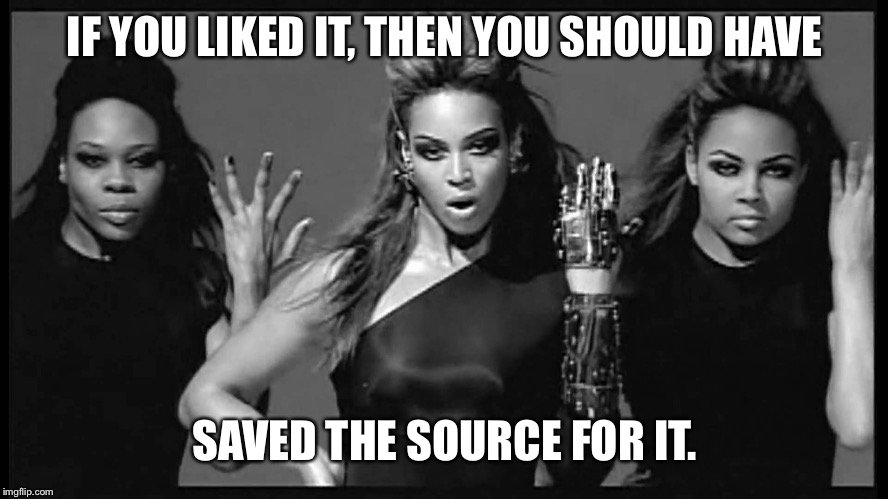
\includegraphics[width=1\textwidth,height=\textheight]{./img/if-you-liked-it-you-should-have-saved-the-source-for-it.jpg}

All important objects or figures should be explicitly saved to file, in
a granular way. This is in contrast to storing them implicitly or
explicitly, as part of an entire workspace, or saving them via the
mouse. These recommendations make useful objects readily available for
use in other scripts or documents, with the additional assurance that
they can be regenerated on-demand. \emph{(future link: the API for an
analysis)}

Saving code -- not workspaces -- is incredibly important because it is
an absolute requirement for reproducibility. Renouncing \texttt{.Rdata}
and restarting R often are not intrinsically important or morally
superior behaviours. They are important because they provide constant
pressure for you to do the right thing: save the source code needed to
create all important artefacts of your analysis.

Below we lay out the concrete measures for adopting this workflow.

\hypertarget{use-an-ide}{%
\section*{Use an IDE}\label{use-an-ide}}
\addcontentsline{toc}{section}{Use an IDE}

When working with R, save your commands in a \texttt{.R} file, a.k.a. a
script, or in \texttt{.Rmd}, a.k.a. an R Markdown document. It doesn't
have to be polished. Just save it!

An
\href{https://en.wikipedia.org/wiki/Integrated_development_environment}{integrated
development environment} (IDE) is critical for making this workflow
pleasant. Without an IDE, you edit your code in one app, copy one or
more lines to the clipboard, then paste that into R, and execute. Over
and over. If this is your life, it is very attractive to type code
directly in R!

Any good IDE offers a powerful, R-aware code editor and provides many
ways to send your code to a running R process (along with other modern
conveniences). This eliminates the temptation to develop code directly
in the R Console. Instead, it becomes easier to do the right thing,
which is to develop code in a \texttt{.R} or \texttt{.Rmd} file.

Some popular IDEs:

\begin{itemize}
\tightlist
\item
  RStudio: download
  \href{https://www.rstudio.com/products/rstudio/download/\#download}{here}
  or (I recommend) run the
  \href{https://www.rstudio.com/products/rstudio/download/preview/}{Preview
  version}
\item
  Emacs + ESS: \url{https://ess.r-project.org}
\item
  vim + Nvim-R: blog post
  \href{https://medium.com/@kadek/turning-vim-into-an-r-ide-cd9602e8c217}{How
  to Turn Vim Into an IDE for R}
\item
  Visual Studio + RTVS:
  \url{https://docs.microsoft.com/en-us/visualstudio/rtvs}
\end{itemize}

Sometimes people resist advice because it's hard to incorporate into
their current workflow and dismiss it as something ``for experts only''.
But this gets the direction of causality backwards: long-time and
professional coders don't do these things because they use an IDE. They
use an IDE because it makes it so much easier to follow best practices.

\hypertarget{always-start-r-with-a-blank-slate}{%
\section*{Always start R with a blank
slate}\label{always-start-r-with-a-blank-slate}}
\addcontentsline{toc}{section}{Always start R with a blank slate}

When you quit R, do not save the workspace to an \texttt{.Rdata} file.
When you launch, do not reload the workspace from an \texttt{.Rdata}
file.

\begin{itemize}
\tightlist
\item
  In RStudio, set this via \emph{Tools \textgreater{} Global Options}.
\end{itemize}

\begin{figure}

{\centering 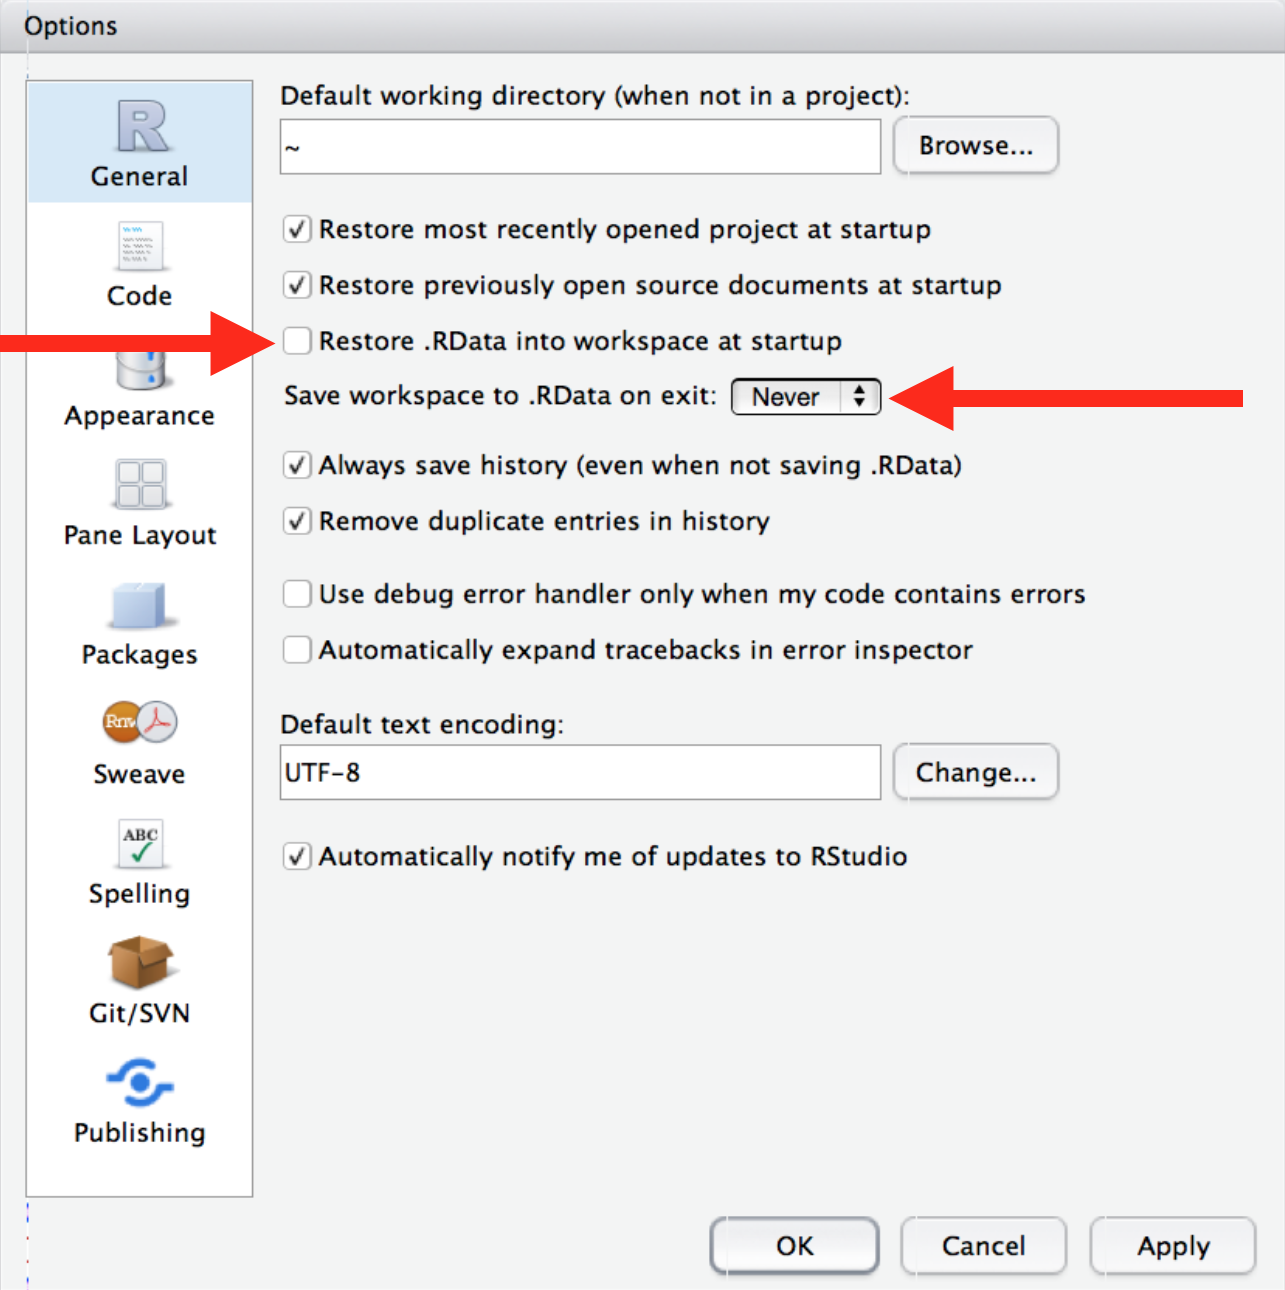
\includegraphics[width=1\textwidth,height=\textheight]{./img/rstudio-workspace.png}

}

\caption{via R for Data Science}

\end{figure}

\begin{verbatim}
FYI: `usethis::use_blank_slate()` prints a reminder about how to do this.
\end{verbatim}

\begin{itemize}
\tightlist
\item
  If you run R from the shell, launch with
  \texttt{R\ -\/-no-save\ -\/-no-restore-data}. You might want to define
  an alias in your \texttt{.bash\_profile}:
  \texttt{alias\ R=\textquotesingle{}R\ -\/-no-save\ -\/-no-restore-data\textquotesingle{}}.
  Learn more by executing \texttt{R\ -\/-help} in a shell.
\end{itemize}

\hypertarget{restart-r-often-during-development}{%
\section*{Restart R often during
development}\label{restart-r-often-during-development}}
\addcontentsline{toc}{section}{Restart R often during development}

\begin{quote}
Have you tried turning it off and then on again?

-- timeless troubleshooting wisdom, applies to everything
\end{quote}

If you use RStudio, use the menu item \emph{Session \textgreater{}
Restart R} or the associated keyboard shortcut Ctrl+Shift+F10 (Windows
and Linux) or Command+Shift+F10 (Mac OS). Additional keyboard shortcuts
make it easy to restart development where you left off, i.e.~to say
``re-run all the code up to HERE'':

\begin{itemize}
\tightlist
\item
  In an R script, use Ctrl+Alt+B (Windows and Linux) or Command+Option+B
  (Mac OS)
\item
  In R markdown, use Ctrl+Alt+P (Windows and Linux) or Command+Option+P
  (Mac OS)
\end{itemize}

If you run R from the shell, use Ctrl+D or \texttt{q()} to quit, then
restart R.

\hypertarget{pre-emptively-handling-a-faq}{%
\subsection*{Pre-emptively handling a
FAQ}\label{pre-emptively-handling-a-faq}}
\addcontentsline{toc}{subsection}{Pre-emptively handling a FAQ}

No, there is no R command you can put at the top of a script to restart
R before executing the rest of the file.

No, this is a not a good reason to build RStudio API hacks into your
scripts. We shall not speak of your favorite trick that starts with
\texttt{.rs.api.*}.

You use a menu or keyboard shortcut to save your code or to re-indent it
or run a spell-checker, right? This is how you should approach
restarting R periodically during the day. It's a workflow task. It does
not belong in your code.

Which brings us to \ldots{}

\hypertarget{rm-list-ls}{%
\section*{\texorpdfstring{What's wrong with
\texttt{rm(list\ =\ ls())}?}{What's wrong with rm(list = ls())?}}\label{rm-list-ls}}
\addcontentsline{toc}{section}{What's wrong with
\texttt{rm(list\ =\ ls())}?}

It's fairly common to see data analysis scripts that begin with this
object-nuking command:

\begin{Shaded}
\begin{Highlighting}[]
\FunctionTok{rm}\NormalTok{(}\AttributeTok{list =} \FunctionTok{ls}\NormalTok{())}
\end{Highlighting}
\end{Shaded}

This is highly suggestive of a non-reproducible workflow.

This line is meant to reset things, either to power-cycle the current
analysis or to switch from one project to another. But there are better
ways to do both:

\begin{itemize}
\tightlist
\item
  To power-cycle the current analysis, restart R! See above.
\item
  To switch from one project to another, either restart R or, even
  better, use an IDE with proper support for projects, where each
  project gets its own R process. See
  \protect\hyperlink{project-oriented-workflow}{Project-oriented
  workflow}.
\end{itemize}

\textbf{The problem with \texttt{rm(list\ =\ ls())} is that, given the
intent, it does not go far enough.} All it does is delete user-created
objects from the global workspace.

Many other changes to the R landscape persist invisibly and can have
profound effects on subsequent development. Any packages that have ever
been attached via \texttt{library()} are still available. Any options
that have been set to non-default values remain that way. Working
directory is not affected (which is, of course, why we see
\texttt{setwd()} so often here too!).

Why does this matter? It makes your script vulnerable to hidden
dependencies on things you ran in this R process before you executed
\texttt{rm(list\ =\ ls())}.

\begin{itemize}
\tightlist
\item
  You might use functions from a package without including the necessary
  \texttt{library()} call. Your collaborator won't be able to run this
  script.
\item
  You might code up an analysis assuming that
  \texttt{stringsAsFactors\ =\ FALSE} but next week, when you have
  restarted R, everything will inexplicably be broken.
\item
  You might write paths relative to some random working directory, then
  be puzzled next month when nothing can be found or results don't
  appear where you expect.
\end{itemize}

The solution is to write every script assuming it will be run in a fresh
R process. The best way to do that is \ldots{} develop scripts in a
fresh R process!

There is nothing inherently evil about \texttt{rm(list\ =\ ls())}. It's
a red flag, because it is indicative of a non-reproducible workflow.
Since it appears to ``work'' \textasciitilde90\% of the time, it's very
easy to deceive yourself into thinking your script is self-contained,
when it is not.

\hypertarget{objects-that-take-a-long-time-to-create}{%
\section*{Objects that take a long time to
create}\label{objects-that-take-a-long-time-to-create}}
\addcontentsline{toc}{section}{Objects that take a long time to create}

Power-cycling your analysis regularly can be very painful if there are
parts that take a long time to execute.

This indicates it's time for a modular approach that breaks the analysis
into natural phases, each with an associated script and outputs.
\emph{(future link: API for an analysis)} Isolate each computationally
demanding step in its own script and write the precious object to file
with
\texttt{saveRDS(my\_precious,\ here("results",\ "my\_precious.rds"))}.
Now you can develop scripts to do downstream work that reload the
precious object via
\texttt{my\_precious\ \textless{}-\ readRDS(here("results",\ "my\_precious.rds"))}.
Breaking an analysis into logical steps, with clear inputs and outputs,
is a good idea anyway.

\hypertarget{automated-workflows}{%
\section*{Automated workflows}\label{automated-workflows}}
\addcontentsline{toc}{section}{Automated workflows}

Various approaches exist for automating a workflow, i.e.~running a set
of scripts in sequence. Many people can get by with low-tech solutions,
such as \href{http://kbroman.org/minimal_make/}{using GNU Make} or even
writing a pseudo-Makefile in R.

If you use one ``controller'' script to run other R scripts or to render
multiple R Markdown documents, it's a good idea to force the use of a
fresh R process for each one. If your controller script is written in R,
consider using the \href{https://callr.r-lib.org}{callr package} to
\texttt{source()} or \texttt{render()} each worker script or
\texttt{.Rmd} in its own R session.

The R package \href{https://ropenscilabs.github.io/drake-manual/}{drake}
is gaining traction as a formal tool for workflow automation (sort of
GNU make, but for R):

\begin{quote}
It analyzes your workflow, skips steps with up-to-date results, and
orchestrates the rest with optional distributed computing.
\end{quote}

\hypertarget{links-to-other-resources}{%
\section*{Links to other resources}\label{links-to-other-resources}}
\addcontentsline{toc}{section}{Links to other resources}

\href{https://stat545.com/r-basics.html}{This page} from
\href{https://stat545.com}{STAT 545} covers some of the same ground, but
aimed at someone quite new to R.

The post
\href{https://www.tidyverse.org/articles/2017/12/workflow-vs-script/}{Project-oriented
workflow} from the \href{https://www.tidyverse.org/articles/}{tidyverse
blog} is an earlier effort to explain why \texttt{rm(list\ =\ ls())} and
\texttt{setwd()} indicate a sub-optimal workflow.

\begin{itemize}
\tightlist
\item
  That lead to a
  \href{https://community.rstudio.com/t/project-oriented-workflow-setwd-rm-list-ls-and-computer-fires/3549/2}{lively
  thread} on \href{https://community.rstudio.com}{community.rstudio.com}
  where lots of useRs share their experience and tricks.
\end{itemize}

\hypertarget{project-oriented-workflow}{%
\chapter{Project-oriented workflow}\label{project-oriented-workflow}}

In @ref(rm-list-ls), we discouraged the habit of starting R scripts with
\texttt{rm(list\ =\ ls())}, because it doesn't actually achieve the
intended goal: to reset things. Restarting R is a better way to
power-cycle.

But what if you want to shift focus from project A to project B?
Restarting R, alone, is not enough. It doesn't change R's working
directory, which is needed if projects A and B live in different
directories, which they should (see @ref(work-in-a-project)). Also, what
if you want to have project A and B available for work at the same time?

My strong recommendation is to use a development tool with first-class
support for projects. But first \ldots{}

\hypertarget{setwd}{%
\section{\texorpdfstring{We need to talk about
\texttt{setwd("path/that/only/works/on/my/machine")}}{We need to talk about setwd("path/that/only/works/on/my/machine")}}\label{setwd}}

A common response to the working directory problem is to set the working
directory at the beginning of each script via \texttt{setwd()}. At the
start of \href{http://stat545.com}{STAT 545}, we see a lot of student
code that looks like this:

\begin{Shaded}
\begin{Highlighting}[]
\FunctionTok{library}\NormalTok{(ggplot2)}
\FunctionTok{setwd}\NormalTok{(}\StringTok{"/Users/jenny/cuddly\_broccoli/verbose\_funicular/foofy/data"}\NormalTok{)}
\NormalTok{df }\OtherTok{\textless{}{-}} \FunctionTok{read.delim}\NormalTok{(}\StringTok{"raw\_foofy\_data.csv"}\NormalTok{)}
\NormalTok{p }\OtherTok{\textless{}{-}} \FunctionTok{ggplot}\NormalTok{(df, }\FunctionTok{aes}\NormalTok{(x, y)) }\SpecialCharTok{+} \FunctionTok{geom\_point}\NormalTok{()}
\FunctionTok{ggsave}\NormalTok{(}\StringTok{"../figs/foofy\_scatterplot.png"}\NormalTok{)}
\end{Highlighting}
\end{Shaded}

The chance of the \texttt{setwd()} command having the desired effect --
making the file paths work -- for anyone besides its author is 0\%. It's
also unlikely to work for the author one or two years or computers from
now. To recreate and perhaps extend this plot, the lucky recipient will
need to hand edit one or more paths to reflect where the project has
landed on their machine.

Hard-wired, absolute paths, especially when sprinkled throughout the
code, make a project brittle. Such code does not travel well across time
or space.

If, after reading this article, you still decide to use \texttt{setwd()}
in your scripts, you should at least be very disciplined about it:

\begin{itemize}
\item
  Only use \texttt{setwd()} at the very start of a file, i.e.~in an
  obvious and predictable place. If someone has to hand-edit all of
  these, make it easy for them.
\item
  Always set working directory to the same thing, namely to the
  top-level of the project (not a subdirectory). Always build subsequent
  paths relative to that. Here's how that looks in the previous example:

\begin{Shaded}
\begin{Highlighting}[]
\FunctionTok{setwd}\NormalTok{(}\StringTok{"/Users/jenny/cuddly\_broccoli/verbose\_funicular/foofy"}\NormalTok{)}

\FunctionTok{library}\NormalTok{(ggplot2)}
\NormalTok{df }\OtherTok{\textless{}{-}} \FunctionTok{read.delim}\NormalTok{(}\StringTok{"data/raw\_foofy\_data.csv"}\NormalTok{)}
\NormalTok{p }\OtherTok{\textless{}{-}} \FunctionTok{ggplot}\NormalTok{(df, }\FunctionTok{aes}\NormalTok{(x, y)) }\SpecialCharTok{+} \FunctionTok{geom\_point}\NormalTok{()}
\FunctionTok{ggsave}\NormalTok{(}\StringTok{"figs/foofy\_scatterplot.png"}\NormalTok{)}
\end{Highlighting}
\end{Shaded}
\end{itemize}

The convention about leaving working directory at the top-level of a
project is tightly connected to topics in @ref(safe-paths).

\hypertarget{if-you-like-setwd-then-carry-on}{%
\subsection{\texorpdfstring{If you like \texttt{setwd()}, then carry
on}{If you like setwd(), then carry on}}\label{if-you-like-setwd-then-carry-on}}

If you use \texttt{setwd("path/that/only/works/on/my/machine")} and it
does not cause you or your collaborators grief, then I am happy for you.
Carry on. This was my practice as well for many years.

But eventually I admitted that this \emph{did} cause me grief whenever I
moved my files, collaborated on an analysis with a colleague, or got a
new computer. Then, as the instructor of
\href{http://stat545.com}{STAT545}, I started to run other people's code
\emph{en masse}. Up to 80 students submitted multiple \texttt{.R} and
\texttt{.Rmd} files each week, riddled with \texttt{setwd()} calls that
required artisanal hand editing by me. This was the straw that broke the
camel's back and made me determined to clearly articulate this problem
and some solutions. You can design this particular aggravation out of
your life.

\hypertarget{dilemma-and-a-solution}{%
\section{Dilemma and a solution}\label{dilemma-and-a-solution}}

Problem statement:

\begin{itemize}
\tightlist
\item
  We want to work on project A with R's working directory set to
  \texttt{path/to/projectA} and on project B with R's working directory
  set to \texttt{path/to/projectB}.
\item
  But we also want to keep code like \texttt{setwd("path/to/projectA")}
  out of our \texttt{.R} scripts.
\end{itemize}

The lowest-tech solution is to simply set working directory yourself,
interactively, at the same time as you restart R, when you switch from
project A to project B. Execute \texttt{setwd("path/to/projectA")}, but
don't bake it into your scripts. This works! But it's aggravating enough
that most people go back to using \texttt{setwd()} anyway and/or are
reluctant to cycle rapidly between projects.

I strongly recommend \protect\hyperlink{use-an-ide}{using an IDE} that
supports a project-based workflow. This eliminates the tension between
your development convenience and the portability of the code.

\hypertarget{work-in-a-project}{%
\section{Organize work into projects (colloquial
definition)}\label{work-in-a-project}}

Here's what I mean by ``work in a project'':

\begin{itemize}
\tightlist
\item
  File system discipline: put all the files related to a single project
  in a designated folder.

  \begin{itemize}
  \tightlist
  \item
    This applies to data, code, figures, notes, etc.
  \item
    Depending on project complexity, you might enforce further
    organization into subfolders.
  \item
    Other common file practices are detailed in \emph{future link: api
    for a project} and \emph{future link: naming files}.
  \end{itemize}
\item
  Working directory intentionality: when working on project A, make sure
  working directory is set to project A's folder.

  \begin{itemize}
  \tightlist
  \item
    Ideally, this is achieved via the development workflow and tooling,
    not by baking absolute paths into the code.
  \end{itemize}
\item
  File path discipline: all paths are relative and, by default, relative
  to the project's folder.
\end{itemize}

These habits are synergistic: you'll get the biggest payoff if you
practice all of them together.

These habits guarantee that the project can be moved around on your
computer or onto other computers and will still ``just work''. I argue
that this is the only practical convention that creates reliable, polite
behavior across different computers or users and over time. This
convention is neither new, nor unique to R.

It's like agreeing that we will all drive on the left or the right. A
hallmark of civilization is following conventions that constrain your
behavior a little, in the name of public safety.

\hypertarget{ide-support-for-projects}{%
\section{IDE support for projects}\label{ide-support-for-projects}}

Projects are a common and very attractive feature of many IDEs
(@ref(use-an-ide)). Again, the practice of organizing work in projects
is not prevalent among long-time coders because they use an IDE. It's
the other way around: one of the attractions of an IDE is that it makes
it easier to exploit development practices that have proven to be useful
across many languages and domains.

I would say an IDE or workflow supports project-oriented work in R if
there's a way to do these things:

\begin{itemize}
\tightlist
\item
  Launch the IDE in project A:

  \begin{itemize}
  \tightlist
  \item
    Starts R.
  \item
    Sets working directory to the project's folder.
  \end{itemize}
\item
  Switch a running instance of the IDE from project A to project B:

  \begin{itemize}
  \tightlist
  \item
    Restarts R.
  \item
    Sets working directory to the project's folder.
  \item
    Optional but nice: restores previously open files, i.e.~pick up
    where you left off.
  \end{itemize}
\item
  Have project A and project B open for simultaneous work:

  \begin{itemize}
  \tightlist
  \item
    Each project gets its own R process, with working directory set
    appropriately.
  \item
    Optional but nice: multiple projects feel like multiple instances of
    the IDE and you can use a conventional method to switch between
    them, e.g.~Command+Tab (Mac OS) or Alt+Tab (Windows).
  \end{itemize}
\end{itemize}

\hypertarget{rstudio-projects}{%
\section{RStudio Projects}\label{rstudio-projects}}

The RStudio IDE has a notion of a (capital ``P'')
\href{https://support.rstudio.com/hc/en-us/articles/200526207-Using-Projects}{Project},
which is a very effective implementation of the (small ``p'') projects
described above.

You can designate a new or existing folder as a Project. All this means
is that RStudio leaves a file, e.g., \texttt{foofy.Rproj}, in the
folder, which is used to store settings specific to that project. Use
\emph{File \textgreater{} New Project \ldots{}} to get started.

Double-click on a \texttt{.Rproj} file to open a fresh instance of
RStudio, with the working directory and file browser pointed at the
project folder.

Once RStudio is running, you can open an existing Project, switch to
another Project, launch a second instance of RStudio in a new or
existing Project, and much more, via various menus and keyboard
shortcuts (more below).

Here's a screenshot of the Mac OS app switcher invoked via Command+Tab,
showing multiple simultaneous instances of RStudio.

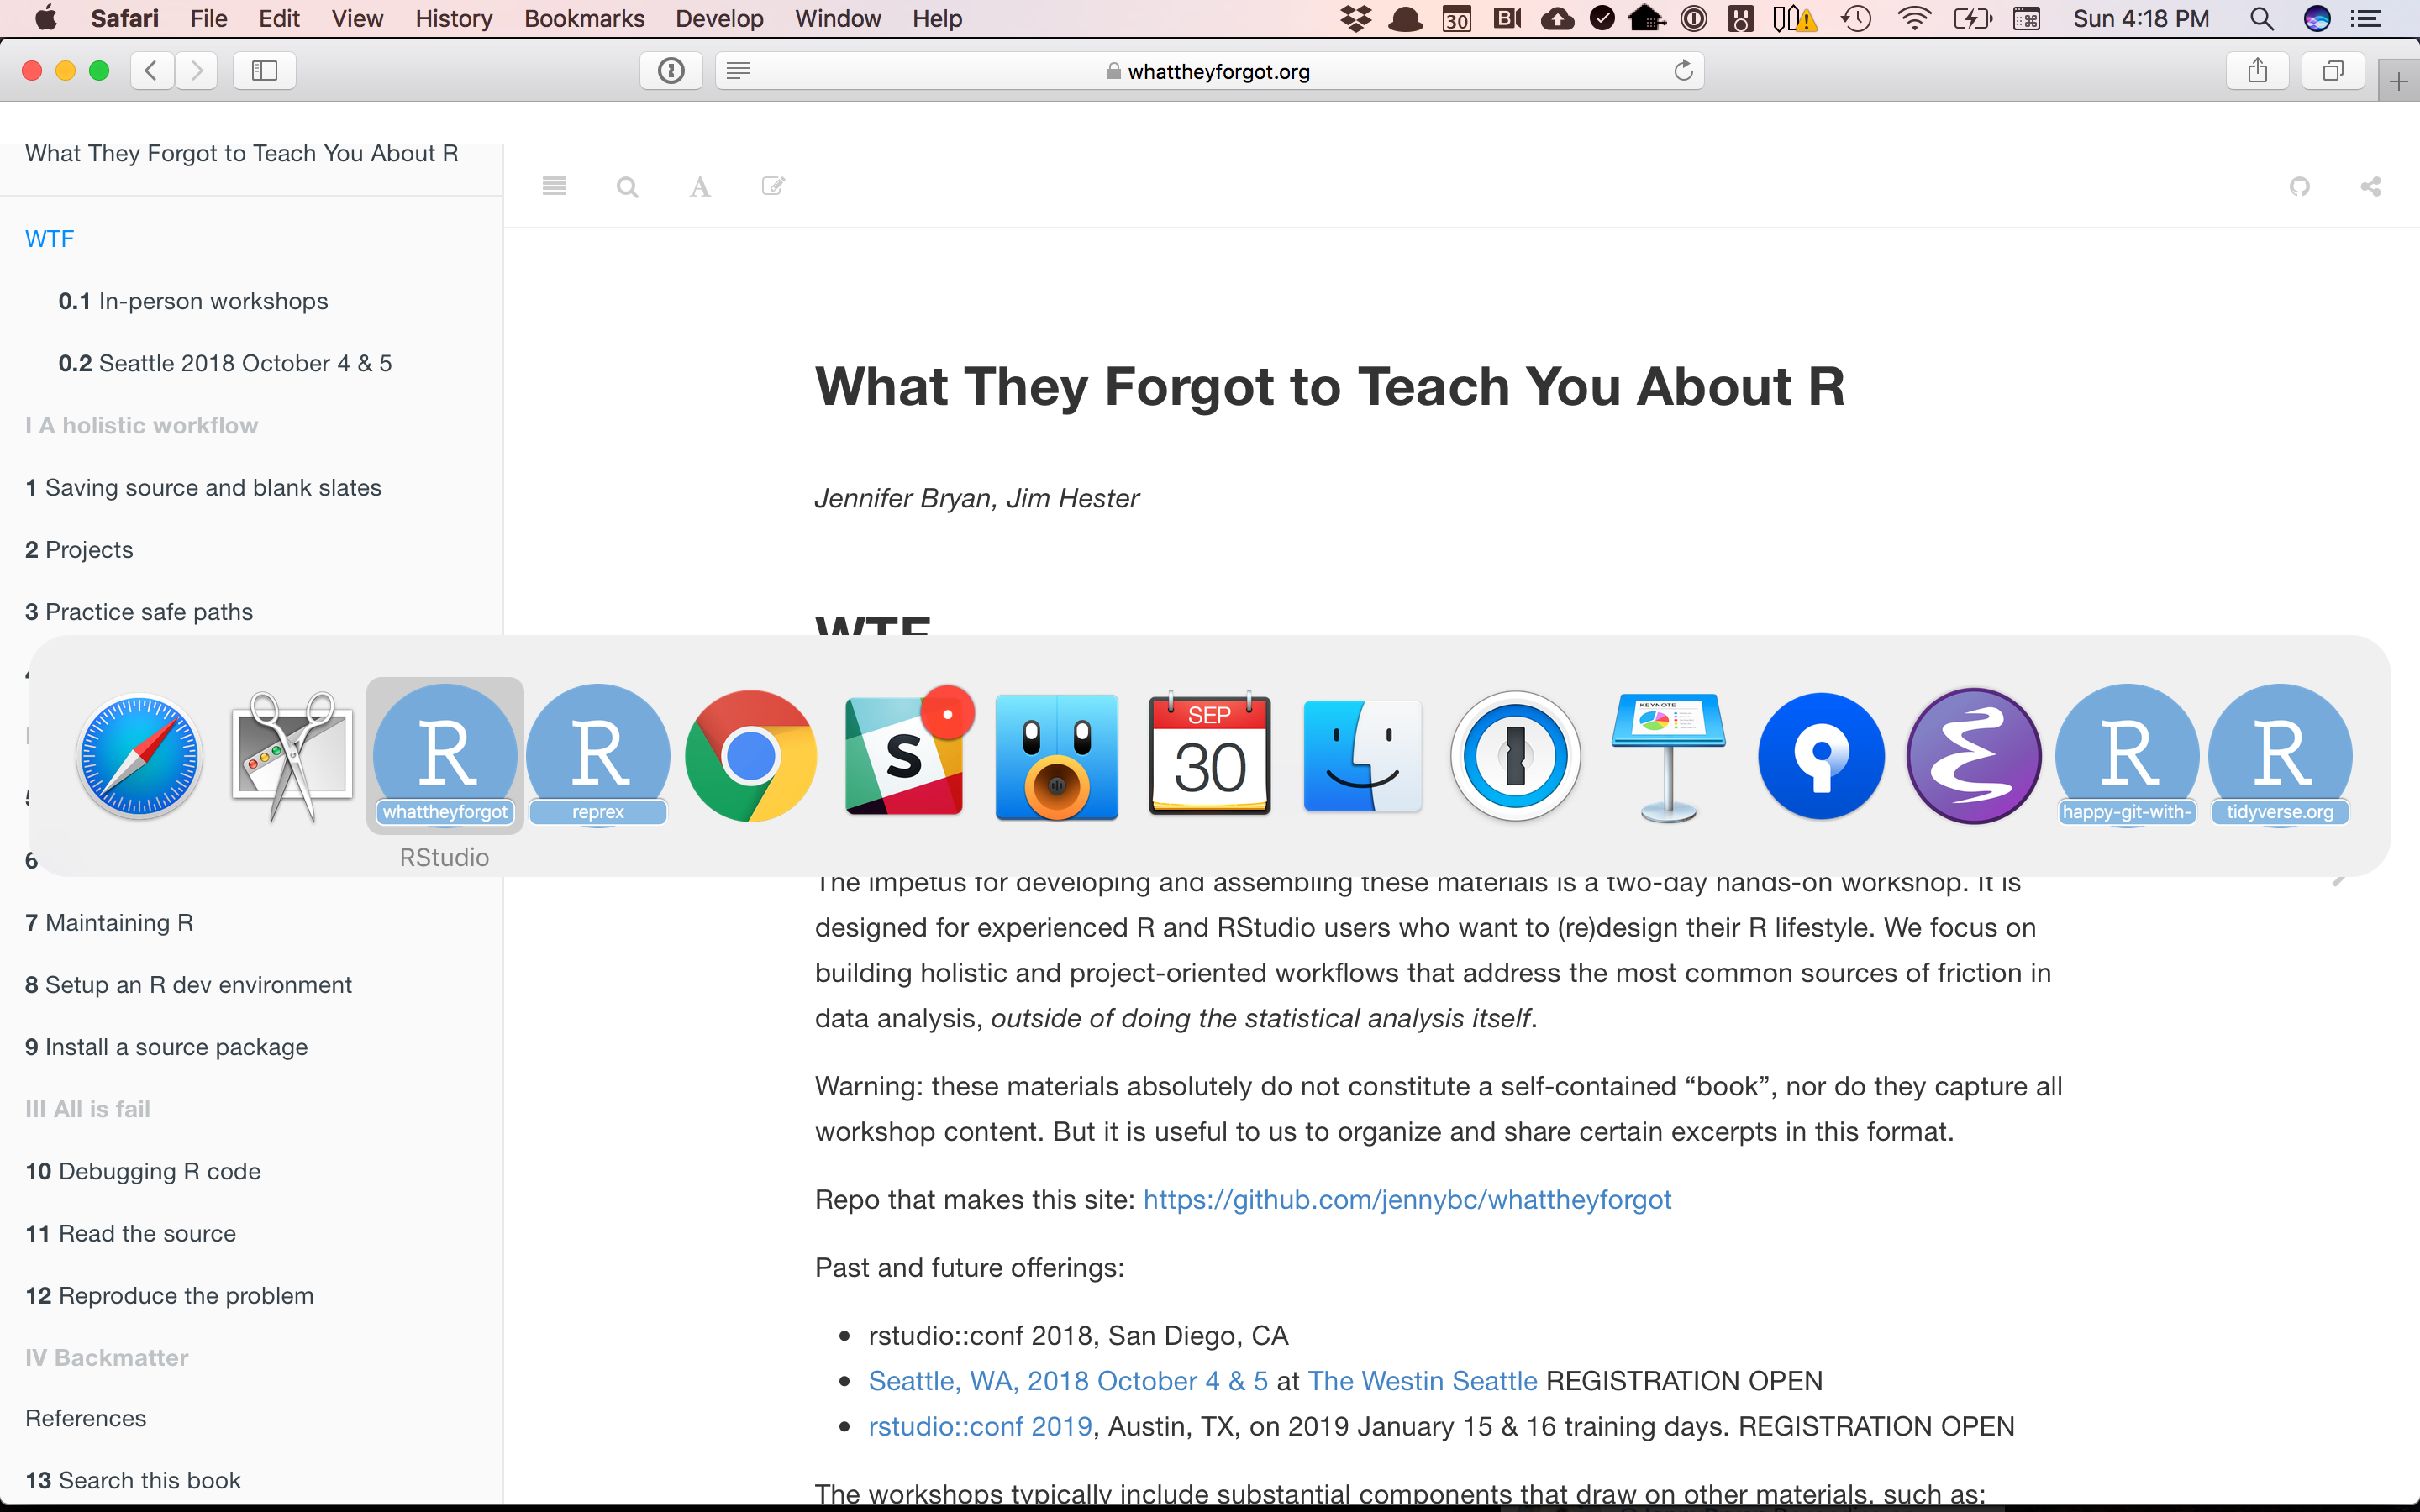
\includegraphics[width=1\textwidth,height=\textheight]{./img/multiple-rstudio-projects.png}

This allows rapid context switching across several projects, such as an
R package, teaching material, and a data analysis. There is no danger of
crosstalk between the projects: each has its own R process, global
workspace, and working directory.

\hypertarget{tricks-for-opening-projects}{%
\subsection{Tricks for opening
Projects}\label{tricks-for-opening-projects}}

Once you decide ``I want to do some work in Project K'', there are
various ways to accelerate the startup process. I'll review a few going
from general and low-tech to more specific.

\textbf{Have a dedicated folder for your Projects.} I keep the vast
majority of my R work in RStudio Projects in the folder
\texttt{\textasciitilde{}/rrr/}. What I call this folder and where I
keep it is not important. The main point is if you have One Main Place
for Projects, then you can go there in Finder or File Explorer and drill
down to the \texttt{.Rproj} file needed to launch any specific project.
You can make the One Main Place more accessible to yourself by putting
it in the Finder's Sidebar (macOS) or in the Navigation Pane (Windows).

\textbf{RStudio knows about recently used Projects.} Once you are in
RStudio, there are several ways to access other Projects you've recently
worked in. In the upper right corner is a drop-down menu with various
Project- and session-related goodies in it.

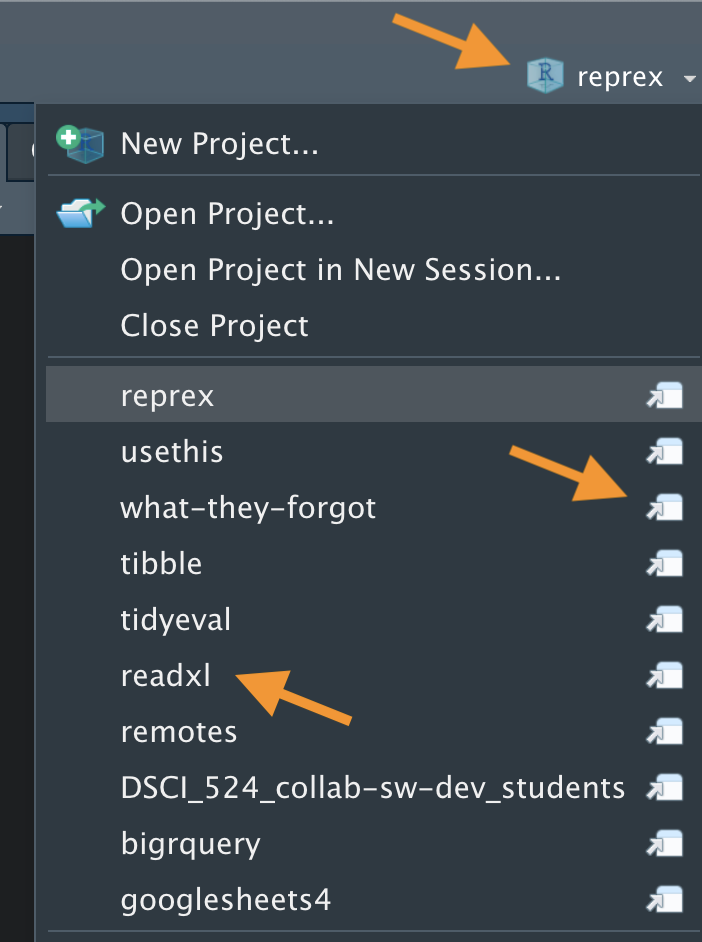
\includegraphics[width=0.5\textwidth,height=\textheight]{./img/rstudio-project-switching.png}

Use the ``arrow and paper'' icon to open a Project in a separate RStudio
instance, while also leaving the Project you're launching it from open.
Click on a Project's name to switch the current RStudio instance from
one Project to another. The \emph{File} menu also offers ways to switch
project or open new, additional instances.

\textbf{Find and Launch Projects with Alfred.} This is a highly specific
app recommendation that only works on macOS, but I'm sure other tools
have a similar capability on macOS and Windows. I use
\href{https://www.alfredapp.com}{Alfred}, which is a macOS application
launcher and general productivity booster, based on a recommendation
from Hadley Wickham.

You will set an Alfred hotkey (I use Option + Space), similar to macOS
Spotlight. The hotkey calls up a search window, where you can summon
apps or files. I've configured Alfred to search preferentially for
\texttt{.Rproj} files here, making it extremely easy to find and launch
RStudio Projects. Here's what happens when I type ``tidy'':

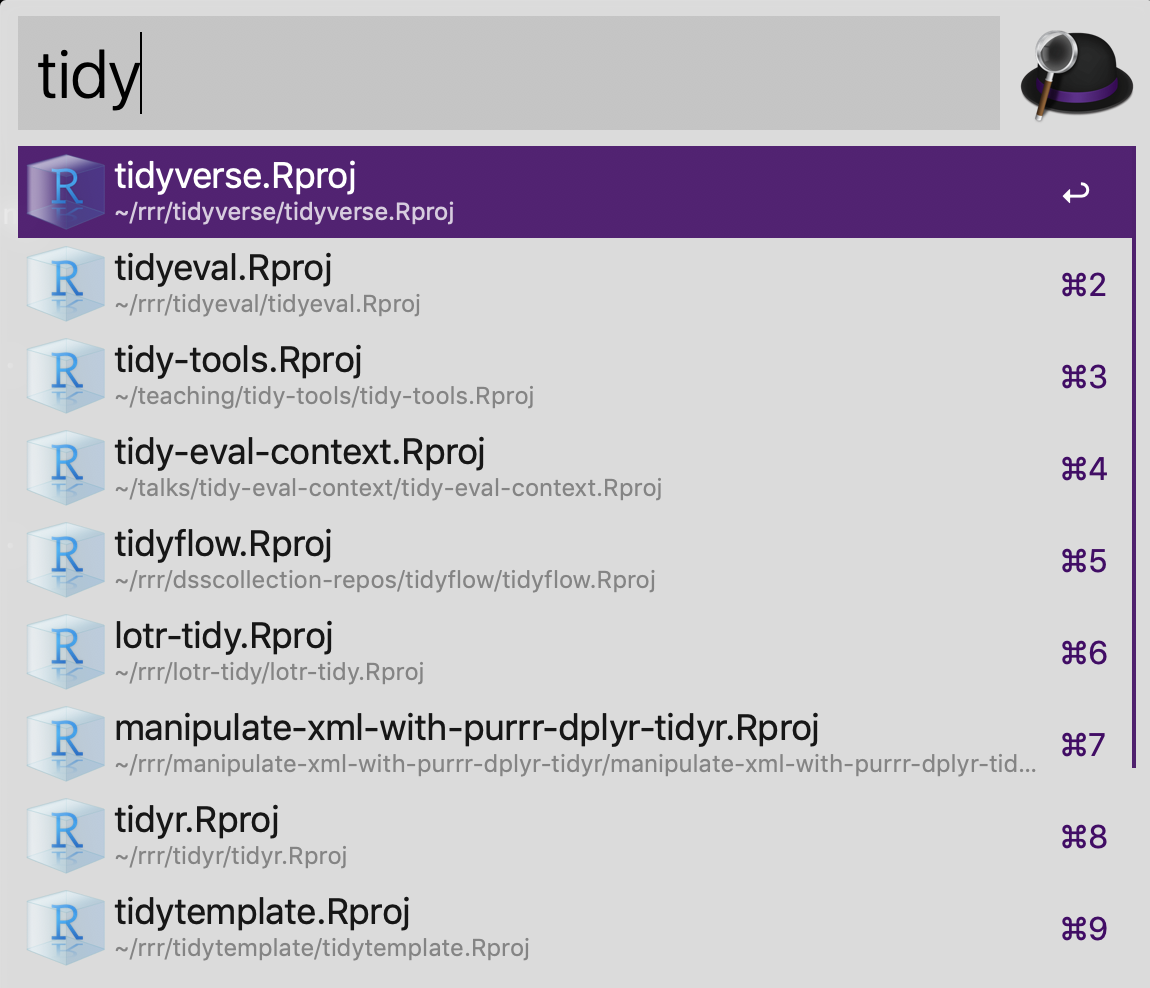
\includegraphics[width=0.5\textwidth,height=\textheight]{./img/alfred-tidy.png}

You can achieve this by ``registering'' the \texttt{.Rproj} file type
with Alfred. Go to Alfred's \emph{Preferences \textgreater{} Features
\textgreater{} Default Results \textgreater{} Advanced\ldots{}}. Drag
any \texttt{.Rproj} file onto this space and then close.

\hypertarget{other-ways-to-work-with-projects}{%
\section{Other ways to work with
projects}\label{other-ways-to-work-with-projects}}

\emph{Aspirational placeholder.}

\emph{Will hopefully sketch project-friendly workflows that are not
RStudio, e.g.~Emacs + ESS. They do exist but I am not expert in them and
an open to input from those who are. Links to well-developed guides
would be best as I don't want to ingest anything I can't maintain.}

\hypertarget{project-specific-shortcuts-on-windows}{%
\subsection{Project-specific shortcuts on
Windows}\label{project-specific-shortcuts-on-windows}}

\emph{still rough}

After installing R, you will have a shortcut to \texttt{Rgui.exe} on
your desktop and/or somewhere on the Start menu file tree, and perhaps
also in the Quick Launch part of the taskbar (Vista and earlier).

Create a copy of this shortcut for each project. Right-click the new
shortcut, select \texttt{Properties...}, and change the `Start in' field
to the folder where the project lives.

Launch R in a project by double-clicking its suitably-prepared shortcut.

Source:

\begin{itemize}
\tightlist
\item
  R for Windows FAQ question
  \href{https://cran.r-project.org/bin/windows/base/rw-FAQ.html\#How-can-I-keep-workspaces-for-different-projects-in-different-directories_003f}{2.10
  How can I keep workspaces for different projects in different
  directories?}
\end{itemize}

\hypertarget{links-to-other-resources-1}{%
\section{Links to other resources}\label{links-to-other-resources-1}}

\href{http://stat545.com/block002_hello-r-workspace-wd-project.html}{This
page} from \href{http://stat545.com/topics.html}{STAT 545} covers some
of the same ground, but aimed at someone quite new to R.

The post
\href{https://www.tidyverse.org/articles/2017/12/workflow-vs-script/}{Project-oriented
workflow} from the \href{https://www.tidyverse.org/articles/}{tidyverse
blog} is an earlier effort to explain why \texttt{rm(list\ =\ ls())} and
\texttt{setwd()} indicate a sub-optimal workflow.

\begin{itemize}
\tightlist
\item
  That lead to a
  \href{https://community.rstudio.com/t/project-oriented-workflow-setwd-rm-list-ls-and-computer-fires/3549/2}{lively
  thread} on \href{https://community.rstudio.com}{community.rstudio.com}
  where lots of useRs share their experience and tricks.
\end{itemize}

\hypertarget{safe-paths}{%
\chapter{Practice safe paths}\label{safe-paths}}

Adapt from \url{https://github.com/jennybc/here_here\#readme}.

Include some coverage of fs.

\hypertarget{use-projects-and-the-here-package}{%
\section{\texorpdfstring{Use projects and the
\href{https://CRAN.R-project.org/package=here}{here
package}}{Use projects and the here package}}\label{use-projects-and-the-here-package}}

How can you avoid \texttt{setwd()} at the top of every script?

\begin{itemize}
\tightlist
\item
  Organize each logical project into a folder on your computer.
\item
  Make sure the top-level folder advertises itself as such. This can be
  as simple as having an empty file named \texttt{.here}. Or, if you use
  RStudio and/or Git, those both leave characteristic files behind that
  will get the job done.
\item
  Use the \texttt{here()} function from the
  \href{https://CRAN.R-project.org/package=here}{here package} to build
  the path when you read or write a file. Create paths relative to the
  top-level directory.
\item
  Whenever you work on this project, launch the R process from the
  project's top-level directory. If you launch R from the shell,
  \texttt{cd} to the correct folder first.
\end{itemize}

To continue our example, start R in the \texttt{foofy} directory,
wherever that may be. Now the code looks like so:

\begin{Shaded}
\begin{Highlighting}[]
\FunctionTok{library}\NormalTok{(ggplot2)}
\FunctionTok{library}\NormalTok{(here)}

\NormalTok{df }\OtherTok{\textless{}{-}} \FunctionTok{read.delim}\NormalTok{(}\FunctionTok{here}\NormalTok{(}\StringTok{"data"}\NormalTok{, }\StringTok{"raw\_foofy\_data.csv"}\NormalTok{))}
\NormalTok{p }\OtherTok{\textless{}{-}} \FunctionTok{ggplot}\NormalTok{(df, }\FunctionTok{aes}\NormalTok{(x, y)) }\SpecialCharTok{+} \FunctionTok{geom\_point}\NormalTok{()}
\FunctionTok{ggsave}\NormalTok{(}\FunctionTok{here}\NormalTok{(}\StringTok{"figs"}\NormalTok{, }\StringTok{"foofy\_scatterplot.png"}\NormalTok{))}
\end{Highlighting}
\end{Shaded}

This will run, with no edits, for anyone who follows the convention
about launching R in the project folder. In fact, it will even work if
R's working directory is anywhere inside the project, i.e.~it will work
from sub-folders. This plays well with knitr/rmarkdown's default
behavior around working directory and in package development/checking
workflows.

Read up on the \href{https://CRAN.R-project.org/package=here}{here
package} to learn about more features, such as additional ways to mark
the top directory and troubleshooting with \texttt{dr\_here()}. I have
also written a \href{https://github.com/jennybc/here_here}{more detailed
paean} to this package before.

\hypertarget{how-to-name-files}{%
\chapter{How to name files}\label{how-to-name-files}}

Convert content from these slides
\url{https://speakerdeck.com/jennybc/how-to-name-files}

\hypertarget{api-for-an-analysis}{%
\chapter{API for an analysis}\label{api-for-an-analysis}}

Prose version of slides 57 - 63 from here:

\url{https://speakerdeck.com/jennybc/zen-and-the-art-of-workflow-maintenance?slide=57}

\part{Personal R Administration}

\begin{figure}[H]

{\centering \includegraphics[width=5.5in,height=3.5in]{./personal-radmin_files/figure-latex/mermaid-figure-1.png}

}

\end{figure}

\hypertarget{part-personal-r-admin}{%
\chapter*{(PART) Personal R Admin}\label{part-personal-r-admin}}
\addcontentsline{toc}{chapter}{(PART) Personal R Admin}

\hypertarget{get-to-know-your-r-installation}{%
\chapter*{Get to know your R
installation}\label{get-to-know-your-r-installation}}
\addcontentsline{toc}{chapter}{Get to know your R installation}

R version, where the executable lives.

Study your package library.

\hypertarget{r-startup}{%
\chapter{R Startup}\label{r-startup}}

R has been designed to be used from shared computing resources such as
linux servers. As a result R's startup offers lots of opportunity for
customization; both for every user of a system as well as for each
individual user. However this flexibility comes at a cost:
\emph{complexity}.

And for sure, R's startup procedures are complex:

\begin{figure}

{\centering \includegraphics{./images/R-startup.svg}

}

\caption{R Startup flowchart -
\href{https://twitter.com/thomasp85/status/961553618196418560}{Thomas
Lin Pedersen}}

\end{figure}

However most R users can ignore the majority of this complexity and
focus on two main files.

\begin{enumerate}
\def\labelenumi{\arabic{enumi}.}
\tightlist
\item
  \protect\hyperlink{renviron}{\texttt{.Renviron}} - which contains
  environment variables to be set in R sessions.
\item
  \protect\hyperlink{rprofile}{\texttt{.Rprofile}} - which contains R
  code to be run in each session.
\end{enumerate}

These files are R specific instances of a broader family of
customization files commonly referred to as
\href{https://www.quora.com/What-are-dotfiles}{dotfiles}. These are used
to tailor the behavior of many programs, particularly those with roots
in the unix command line.

Many people store their \href{https://dotfiles.github.io/}{dotfiles on
GitHub} and a great way to find inspiration for what you can do with
them is to browse other people's dotfile repositories.

One way to find R specific dotfiles is to do a
\href{https://github.com/search?q=filename\%3A.Rprofile+interactive\&type=Code}{GitHub
search for filename:.Rprofile}.

\hypertarget{renviron}{%
\section{\texorpdfstring{\texttt{.Renviron}}{.Renviron}}\label{renviron}}

The \texttt{.Renviron} file is most useful for defining sensitive
information such as API keys (such as GitHub or twitter) as well as R
specific environment variables like the history size
(\texttt{R\_HISTSIZE=100000}) and default library locations
\texttt{R\_LIBS\_USER}.

The \texttt{.Renviron} file contains lists of environment variables to
set. This is \emph{not} R code, it uses a format similar to that used on
the command line shell.

The easiest way to edit \texttt{.Renviron} is by running
\texttt{usethis::edit\_r\_environ()}.

A simple example of a \texttt{.Renviron} file is

\begin{Shaded}
\begin{Highlighting}[]
\NormalTok{R\_HISTSIZE=100000}
\NormalTok{GITHUB\_PAT=abc123}
\NormalTok{R\_LIBS\_USER=\textasciitilde{}/R/\%p/\%v}
\end{Highlighting}
\end{Shaded}

\begin{rmdinfo}
\href{https://raw.githubusercontent.com/rstats-wtf/wtf-startup/master/01_startup_spartan.R}{Try
the activity}
\texttt{usethis::use\_course("rstd.io/wtf-source-package")}

to learn how to set a GitHub PAT to your \texttt{.Renviron} and then use
it with \texttt{usethis::use\_github()} to upload a project to GitHub.
\end{rmdinfo}

\hypertarget{rprofile}{%
\section{\texorpdfstring{\texttt{.Rprofile}}{.Rprofile}}\label{rprofile}}

The \texttt{.Rprofile} file contains R code to be run when R starts up.
It is run after the \texttt{.Renviron} file is sourced. Typically
\texttt{.Rprofile} is located in the users' home directory
(\texttt{\textasciitilde{}/.Rprofile}), however a different location can
be configured by setting the \texttt{R\_PROFILE\_USER} environment
variable.

The easiest way to edit \texttt{.Rprofile} is by running
\texttt{usethis::edit\_r\_profile()}.

Some common things people often add to their \texttt{.RProfile}

\begin{enumerate}
\def\labelenumi{\arabic{enumi}.}
\tightlist
\item
  Set a default CRAN mirror
\item
  Write a welcome message
\item
  Customize their R prompt
\item
  Change options, screen width, numeric display
\item
  Load frequently used packages (but be very careful)
\item
  Aliases / shortcuts for frequently used functions
\end{enumerate}

\hypertarget{reproducibility}{%
\subsection{Reproducibility}\label{reproducibility}}

A good rule of thumb is you should only put things in your
\texttt{.Rprofile} that you run interactively in the R terminal. If it
ever appears in a R script or R Markdown file it should \emph{not} be in
your \texttt{.Rprofile}.

If you set these options in your \texttt{.Rprofile}, then try to run one
of your scripts on another system without your \texttt{.Rprofile} it
will no longer be reproducible. Some problematic examples are loading
packages \emph{used} in analysis (such as \texttt{dplyr} or
\texttt{ggplot2}) or changing default options which change the
\emph{value} of outputs, such as
\texttt{options(stringsAsFactors\ =\ FALSE)}.

In addition because the \texttt{.Rprofile} is run by \emph{every} R
process (including those started by R itself) it is important to guard
most of the code with \texttt{interactive()}, so it is only run in
interactive sessions (sessions you are controlling with a terminal).

A simple example of a \texttt{.Rprofile} is

\begin{Shaded}
\begin{Highlighting}[]
\FunctionTok{options}\NormalTok{(}\AttributeTok{repos =} \FunctionTok{c}\NormalTok{(}\AttributeTok{CRAN =} \StringTok{"https://cran.rstudio.org"}\NormalTok{))}

\ControlFlowTok{if}\NormalTok{ (}\FunctionTok{interactive}\NormalTok{()) \{}
  \FunctionTok{options}\NormalTok{(}\AttributeTok{width =} \DecValTok{120}\NormalTok{)}
\NormalTok{\}}
\end{Highlighting}
\end{Shaded}

\begin{rmdinfo}
\href{https://raw.githubusercontent.com/rstats-wtf/wtf-startup/master/02_startup_spartan.R}{Try
the activity}
\texttt{usethis::use\_course("rstd.io/wtf-source-package")}

to learn how to create a \texttt{.Rprofile} with a default CRAN
repository and add a startup message to it.
\end{rmdinfo}

\hypertarget{disabling-startup-files}{%
\section{Disabling startup files}\label{disabling-startup-files}}

You can run R without any startup files by using the
\texttt{-\/-vanilla} argument when starting R. In RStudio you can do
this by checking the option
\texttt{Project\ Options\ -\textgreater{}\ Disable\ .Rprofile\ execution\ on\ session\ start\ /\ resume}.
You can also selectively disable only the user or site
\texttt{.Rprofile} with \texttt{-\/-no-init-file} and
\texttt{-\/-no-site-file} respectively, and disable the environment
files with \texttt{-\/-no-environ}.

\begin{rmdwarning}
Both \texttt{.Renviron} and \texttt{.Rprofile} \emph{must} end with a
newline character. If they do not the last line with be ignored without
a warning or error.
\end{rmdwarning}

\hypertarget{maintaining-r}{%
\chapter{Maintaining R}\label{maintaining-r}}

\hypertarget{how-to-upgrade-an-installed-package-to-the-latest-version.}{%
\section{How to upgrade an installed package to the latest
version.}\label{how-to-upgrade-an-installed-package-to-the-latest-version.}}

Sometimes you would like to upgrade a particular package to the latest
available version. Often this is because you have heard about a new
feature, or maybe you have run into a bug that may have been fixed.

\hypertarget{in-rstudio}{%
\subsection{In RStudio}\label{in-rstudio}}

\begin{figure}

{\centering 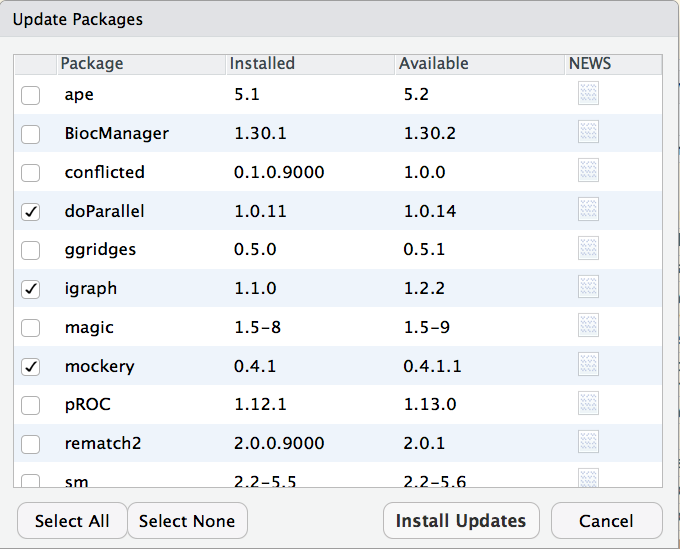
\includegraphics{./images/rstudio-update.png}

}

\caption{RStudio has an update dialog (Packages Tab -\textgreater{}
Update). Check packages to update them}

\end{figure}

\hypertarget{r-terminal}{%
\subsection{R terminal}\label{r-terminal}}

Devtools has a function \texttt{update\_packages()} which will upgrade a
package (from the same source) for \emph{any} CRAN or development
package.

\texttt{devtools::update\_packages("pkgname")}

In addition if the given package is \emph{not} already installed it will
install it.

\hypertarget{how-to-upgrade-all-out-of-date-packages}{%
\section{How to upgrade all out-of-date
packages}\label{how-to-upgrade-all-out-of-date-packages}}

\hypertarget{in-rstudio-1}{%
\subsection{In RStudio}\label{in-rstudio-1}}

\begin{figure}

{\centering 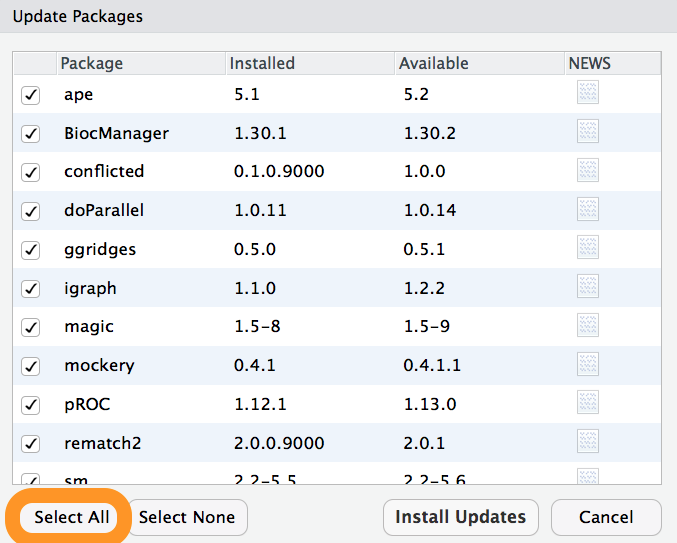
\includegraphics{./images/rstudio-update-all.png}

}

\caption{RStudio also allows you to update all packages (Packages Tab
-\textgreater{} Update -\textgreater{} Select All)}

\end{figure}

\hypertarget{cran-packages}{%
\subsection{CRAN packages}\label{cran-packages}}

\texttt{devtools::update\_packages(TRUE)}

\hypertarget{how-to-downgrade-a-package}{%
\section{How to downgrade a package}\label{how-to-downgrade-a-package}}

First if unsure what version -\textgreater{}
\href{https://cran.r-project.org/web/packages/devtools/index.html}{CRAN
page} -\textgreater{}
\href{https://cran.r-project.org/src/contrib/Archive/devtools/}{pkgname
archive}

\begin{Shaded}
\begin{Highlighting}[]
\NormalTok{devtools}\SpecialCharTok{::}\FunctionTok{install\_version}\NormalTok{(}\StringTok{"devtools"}\NormalTok{, }\StringTok{"1.13.3"}\NormalTok{)}
\end{Highlighting}
\end{Shaded}

\hypertarget{how-to-transfer-your-library-when-updating-r}{%
\section{How to transfer your library when updating
R}\label{how-to-transfer-your-library-when-updating-r}}

Often you will not need to do anything when updating R. For `patch' R
versions, the `z' in `x.y.z' the R core developers ensure package
compatibility across versions. So if you are updating from R 3.5.0 to R
3.5.1 you can use the same packages you are currently using.

For `minor' version changes, the `y' in `x.y.z' the package interface
\emph{can} change, so packages need to be re-installed.

\begin{rmdwarning}
You may see some suggestions that you can just copy your packages even
when the `minor' version changes. \textbf{DO NOT DO THIS}. While it may
work some (even most) of the time, R-core does not guarantee
compatibility between these versions and things could break (even break
silently).
\end{rmdwarning}

I suggest you keep the packages R comes with (base and recommended)
packages separate from the rest of your packages. This makes it easy to
re-install R if needed without touching your CRAN packages. You also
want to make sure the package library is specific to the minor version
of R.

\texttt{R\_LIBS\_USER} is actually set by default to this scheme, (to
\texttt{\textasciitilde{}/R/win-library/x.y} on Windows and
\texttt{\textasciitilde{}/Library/R/x.y/library} on macOS) but the
directory may not already exist, so one option is just to create this
directory (\texttt{fs::dir\_create(Sys.getenv("R\_LIBS\_USER"))}).

You can also alternatively set \texttt{R\_LIBS\_USER} to a different
path; but make sure to include the \texttt{\%v} wildcard.
e.g.~\texttt{\textasciitilde{}/R/library/\%v}. The \texttt{\%v} is
automatically expanded to the major and minor version of R, so with R
3.5.1 this path becomes
\texttt{\textasciitilde{}/Library/R/3.5/library}. See
\protect\hyperlink{renviron}{Renviron} for how to edit your
\texttt{.Renviron} file.

\begin{rmdwarning}
Paths in \texttt{R\_LIBS\_USER} are only used if the directories they
specify actually exist. So in addition to adding \texttt{R\_LIBS\_USER}
to your \texttt{.Renviron} you need to create the directory as well.
\end{rmdwarning}

Once this is setup, the process for transferring your package library
becomes. (assumes \texttt{R\_LIBS\_USER} is set to
\texttt{\textasciitilde{}/Library/R/3.5/library}).

\begin{Shaded}
\begin{Highlighting}[]
\CommentTok{\# Install new version of R (lets say 3.5.0 in this example)}

\CommentTok{\# Create a new directory for the version of R}
\NormalTok{fs}\SpecialCharTok{::}\FunctionTok{dir\_create}\NormalTok{(}\StringTok{"\textasciitilde{}/Library/R/3.5/library"}\NormalTok{)}

\CommentTok{\# Re{-}start R so the .libPaths are updated}

\CommentTok{\# Lookup what packages were in your old package library}
\NormalTok{pkgs }\OtherTok{\textless{}{-}}\NormalTok{ fs}\SpecialCharTok{::}\FunctionTok{path\_file}\NormalTok{(fs}\SpecialCharTok{::}\FunctionTok{dir\_ls}\NormalTok{(}\StringTok{"\textasciitilde{}/Library/R/3.4/library"}\NormalTok{))}

\CommentTok{\# Filter these packages as needed}

\CommentTok{\# Install the packages in the new version}
\FunctionTok{install.packages}\NormalTok{(pkgs)}
\end{Highlighting}
\end{Shaded}

\hypertarget{install-a-source-package}{%
\chapter{Install a source package}\label{install-a-source-package}}

The most common type of package you install is a \textbf{binary}
package. Packages released on CRAN are built as pre-compiled binaries.

However often it is useful to install packages which do not have a
pre-built binary version available. This allows you to install
development versions not yet released on CRAN, as well as older versions
of released packages. It also lets you build your own packages locally.

To install a source package you will need to
\protect\hyperlink{setup-an-r-dev-environment}{setup a development
environment}.

There are a few main functions used to install source packages.

\begin{itemize}
\tightlist
\item
  \texttt{devtools::install\_dev()} to install the latest development
  version of a CRAN package. \footnote{This will only work if the
    package includes a link to the development location in the package
    DESCRIPTION}
\item
  \texttt{devtools::install\_github()} to install a package directly
  from GitHub, even if it is not on CRAN.
\item
  \texttt{devtools::install\_version()} to install previously released
  CRAN versions of a package.
\end{itemize}

For example \texttt{devtools::install\_dev("dplyr")} will install the
development version of dplyr.
\texttt{devtools::install\_github("jimhester/lookup")} will install
Jim's lookup package (which is not on CRAN), and
\texttt{devtools::install\_version("readr",\ "1.0.0")} will install
readr 1.0.0.

It is also possible to \href{https://happygitwithr.com/fork.html}{fork,
clone and work with a package directly} then use
\texttt{devtools::install()} and \texttt{devtools::load\_all()} to work
with the package locally like you would with a package you have created
yourself.

\hypertarget{installation-to-a-temporary-library}{%
\section{Installation to a temporary
library}\label{installation-to-a-temporary-library}}

It is sometimes useful to install packages to a temporary library, so
that they don't affect your normal packages. This can be done by using
the \texttt{lib} argument to the devtools install functions, then using
\texttt{lib.loc} in \texttt{library()} when you load the package.

\begin{Shaded}
\begin{Highlighting}[]
\FunctionTok{library}\NormalTok{(devtools)}

\NormalTok{tmp\_lib }\OtherTok{\textless{}{-}} \StringTok{"\textasciitilde{}/tmp/tmp\_library"}
\FunctionTok{dir.create}\NormalTok{(tmp\_lib)}

\NormalTok{devtools}\SpecialCharTok{::}\FunctionTok{install\_github}\NormalTok{(}\StringTok{"dill/beyonce"}\NormalTok{, }\AttributeTok{lib =}\NormalTok{ tmp\_lib)}

\DocumentationTok{\#\# restart R}

\DocumentationTok{\#\# explicitly load the affected packages from the temporary library}
\FunctionTok{library}\NormalTok{(beyonce, }\AttributeTok{lib.loc =}\NormalTok{ tmp\_lib)}

\DocumentationTok{\#\# your experimentation goes here}

\DocumentationTok{\#\# done? clean up!}
\FunctionTok{unlink}\NormalTok{(tmp\_lib, }\AttributeTok{recursive =} \ConstantTok{TRUE}\NormalTok{)}
\end{Highlighting}
\end{Shaded}

\begin{rmdinfo}
\href{https://raw.githubusercontent.com/jimhester/wtf-source-package/master/01_source-package_spartan.R}{Try
the activity}:
\texttt{usethis::use\_course("rstd.io/wtf-source-package")}

To practice installing various types of source packages.
\end{rmdinfo}

\part{All is Fail}

\hypertarget{part-all-is-fail}{%
\chapter*{(PART) All is fail}\label{part-all-is-fail}}
\addcontentsline{toc}{chapter}{(PART) All is fail}

\hypertarget{debugging-r-code}{%
\chapter*{Debugging R code}\label{debugging-r-code}}
\addcontentsline{toc}{chapter}{Debugging R code}

R scripts are great things, when they work. What are some strategies you
can use when things go sideways and an error occurs in your script?

\hypertarget{debugging-your-own-code}{%
\section*{Debugging your own code}\label{debugging-your-own-code}}
\addcontentsline{toc}{section}{Debugging your own code}

The most common case you will run into a bug is when writing new code
yourself. Often the mistake is obvious and easily fixed, but sometimes
it only appears after multiple levels of calls and is harder to
diagnose. There are a few common strategies to use when debugging your
own code.

\begin{itemize}
\tightlist
\item
  Use \texttt{traceback()} to determine where a given error is
  occurring.
\item
  Output diagnostic information in code with \texttt{print()},
  \texttt{cat()} or \texttt{message()} statements.
\item
  Use \texttt{browser()} to open an interactive debugger before the
  error
\item
  Use \texttt{debug()} to automatically open a debugger at the start of
  a function call.
\item
  Use \texttt{trace()} to start a debugger at a location inside a
  function.
\end{itemize}

\hypertarget{traceback}{%
\subsection*{traceback()}\label{traceback}}
\addcontentsline{toc}{subsection}{traceback()}

The \texttt{traceback()} function can be used to print a summary of how
your program arrived at the error. This is also called a call stack,
stack trace or backtrace.

In R this gives you each call that lead up to the error, which can be
very useful for determining what lead to the error.

You can use \texttt{traceback()} in two different ways, either by
calling it immediately after the error has occurred.

\begin{Shaded}
\begin{Highlighting}[]
\NormalTok{f }\OtherTok{\textless{}{-}} \ControlFlowTok{function}\NormalTok{(x) x }\SpecialCharTok{+} \DecValTok{1}
\NormalTok{g }\OtherTok{\textless{}{-}} \ControlFlowTok{function}\NormalTok{(x) }\FunctionTok{f}\NormalTok{(x)}
\FunctionTok{g}\NormalTok{(}\StringTok{"a"}\NormalTok{)}
\end{Highlighting}
\end{Shaded}

\begin{verbatim}
#> Error in x + 1 : non-numeric argument to binary operator
\end{verbatim}

\begin{Shaded}
\begin{Highlighting}[]
\FunctionTok{traceback}\NormalTok{()}
\end{Highlighting}
\end{Shaded}

\begin{verbatim}
#> 2: f(x) at #1
#> 1: g("a")
\end{verbatim}

Or by using \texttt{traceback()} as an error handler, which will call it
immediately on any error. (You could even put this in your
\protect\hyperlink{rprofile}{\texttt{.Rprofile}})

\begin{Shaded}
\begin{Highlighting}[]
\FunctionTok{options}\NormalTok{(}\AttributeTok{error =}\NormalTok{ traceback)}
\FunctionTok{g}\NormalTok{(}\StringTok{"a"}\NormalTok{)}
\end{Highlighting}
\end{Shaded}

\begin{verbatim}
#> Error in x + 1 : non-numeric argument to binary operator
#> 2: f(x) at #1
#> 1: g("a")
\end{verbatim}

\hypertarget{print}{%
\subsection*{\texorpdfstring{\texttt{print()}}{print()}}\label{print}}
\addcontentsline{toc}{subsection}{\texttt{print()}}

Once you know where an error occurs it is then helpful to know why.
Often errors occur because functions are given inputs their authors did
not expect, so it is useful to print the value of objects during
execution.

The most basic way to do this is to sprinkle messages throughout your
code, with \texttt{print()} or \texttt{str()}. \texttt{str()} is often
more useful because it gives more detail into the exact structure of an
object, which may not be the structure you expect it to be.

The main downsides to the print approach is you often have to add them
in multiple places to narrow down the error, and you cannot further
investigate the object.

\hypertarget{browser}{%
\subsection*{\texorpdfstring{\texttt{browser()}}{browser()}}\label{browser}}
\addcontentsline{toc}{subsection}{\texttt{browser()}}

A more sophisticated debugging method is to put a call to
\texttt{browser()} in your code. This will stop execution at that point
and open R's interactive debugger. In the debugger you can run any R
command to look at objects in the current environment, modify them and
continue executing.

Some useful things to do are

\begin{enumerate}
\def\labelenumi{\arabic{enumi}.}
\tightlist
\item
  Use \texttt{ls()} to determine what objects are available in the
  current environment. This allows you to see exactly what things you
  can examine.
\item
  Use \texttt{str()}, \texttt{print()} etc. to examine the objects
\item
  Use \texttt{n} to evaluate the next statement. Use \texttt{s} to
  evaluate the next statement, but step into function calls.
\item
  Use \texttt{where} to print a \protect\hyperlink{traceback}{stack
  trace}
\item
  Use \texttt{c} to leave the debugger and continue execution
\item
  Use \texttt{Q} to exit the debugger and return to the R prompt.
\end{enumerate}

\hypertarget{debugging-in-rstudio}{%
\section*{Debugging in RStudio}\label{debugging-in-rstudio}}
\addcontentsline{toc}{section}{Debugging in RStudio}

\hypertarget{editor-breakpoints}{%
\subsection*{Editor breakpoints}\label{editor-breakpoints}}
\addcontentsline{toc}{subsection}{Editor breakpoints}

RStudio provides some additional tooling for debugging over using R on
the command line. First you can set an editor breakpoint by clicking to
the left of the line number in the source file, or by pressing
\texttt{Shift+F9} with your cursor on the line. A breakpoint is
equivalent to a \texttt{browser()} call, but you avoid needing to change
your code like \texttt{browser()}.

\includegraphics{https://support.rstudio.com/hc/en-us/article_attachments/201608458/editor-breakpoint.png}

\hypertarget{stopping-on-error}{%
\subsection*{Stopping on error}\label{stopping-on-error}}
\addcontentsline{toc}{subsection}{Stopping on error}

If you are trying to hunt down a particular error it is often useful to
have RStudio enter the debugger when it occurs. You can control the
error behavior with
(\texttt{Debug\ -\textgreater{}\ On\ Error\ -\textgreater{}\ Error\ Inspector}).

\includegraphics{https://support.rstudio.com/hc/en-us/article_attachments/201608428/break-in-code.png}

\hypertarget{debugging-console}{%
\subsection*{Debugging console}\label{debugging-console}}
\addcontentsline{toc}{subsection}{Debugging console}

\includegraphics{https://support.rstudio.com/hc/en-us/article_attachments/201608408/console-window.png}

The RStudio debugging console has a few buttons to make debugging a
little nicer, From left to right they are, next (equivalent to
\texttt{n}), step info (\texttt{s}), continue (\texttt{c}) and Stop
(\texttt{Q}).

\hypertarget{debugging-others-code}{%
\section*{Debugging others' code}\label{debugging-others-code}}
\addcontentsline{toc}{section}{Debugging others' code}

When the error is occurring outside of your own code it is also useful
to be able to debug the code. In this case you \emph{could} download the
package code locally and debug it like you would with your own code
above by adding \texttt{print()} and / or \texttt{browser()} calls.
Because R and most R packages are open source this is a perfectly viable
option and one I often do myself. However depending on the package this
can sometimes be challenging, particularly for those packages which come
with R itself.

The other option is to use additional functions which allow you to start
a browser in existing functions, \texttt{recover()}, \texttt{debug()},
\texttt{trace()} .

\hypertarget{recover}{%
\subsection*{\texorpdfstring{\texttt{recover()}}{recover()}}\label{recover}}
\addcontentsline{toc}{subsection}{\texttt{recover()}}

\texttt{recover()} is not used directly, instead it is used as an error
handler, by calling \texttt{options(error\ =\ recover)}. You can also
use other functions, such as \texttt{browser()} as an error handler,
which will start the debugger automatically when there is an error.

The benefit to \texttt{recover()} over using
\texttt{options(error\ =\ browser)} is that you can browse on any of the
call stack, not just where the error occurred. Often the issue is most
easily diagnosed in calls higher on the stack than immediately where the
error occurred.

When \texttt{recover()} is called it prints a list of the current calls,
with a prompt to select which you want to browse in. Then a debugging
session is started at that location.

\begin{rmdinfo}
\href{https://raw.githubusercontent.com/jimhester/wtf-debugging/master/01_debugging_spartan.R}{Try
activity 1} \texttt{usethis::use\_course("rstd.io/wtf-debugging")}
\href{https://raw.githubusercontent.com/jimhester/wtf-debugging/master/02_debugging_spartan.R}{Try
activity 2} \texttt{usethis::use\_course("rstd.io/wtf-debugging")}

to practice debugging errors using the tools described
\end{rmdinfo}

\hypertarget{debug}{%
\subsection*{\texorpdfstring{\texttt{debug()}}{debug()}}\label{debug}}
\addcontentsline{toc}{subsection}{\texttt{debug()}}

If you have control of the code (because you are the one writing it),
using \texttt{browser()} is generally the most convenient way to enter
the debugger. However if the error is occurring in code in a package
what options do you have?

This is where the \texttt{debug()} function is useful, it will open the
R debugger on any function, including those in packages.

\begin{Shaded}
\begin{Highlighting}[]
\FunctionTok{debug}\NormalTok{(ggplot2}\SpecialCharTok{::}\NormalTok{ggplot)}
\end{Highlighting}
\end{Shaded}

Use can use the \texttt{::} syntax to find `exported' functions in a
package, but there is also a way to access \emph{any} function,
including un-exported ones, \texttt{:::}.

\begin{Shaded}
\begin{Highlighting}[]
\FunctionTok{debug}\NormalTok{(ggplot2}\SpecialCharTok{:::}\NormalTok{set\_last\_plot)}
\end{Highlighting}
\end{Shaded}

\texttt{undebug()} is used to remove the debugging code.

\hypertarget{trace}{%
\subsection*{\texorpdfstring{\texttt{trace()}}{trace()}}\label{trace}}
\addcontentsline{toc}{subsection}{\texttt{trace()}}

\texttt{debug()} is very useful, but one drawback is it always executes
the first time a function is called. What can you do if the bug only
happens the 100th time a function is called?

\texttt{trace()} is a more flexible version of \texttt{debug()} that not
only lets you start a debugger at the start of a function, it lets you
insert \emph{any} code at \emph{any} location in a function. The
downside to this power and flexibility is that \texttt{trace()} is
comparatively harder to use than \texttt{debug()}.

If called with no additional arguments \texttt{trace()} simply prints a
message when the function is entered.

If called with a function as the second argument this inserts the
function at the start of the function. \texttt{trace(fun,\ browser)} is
functionally equivalent to \texttt{debug(fun)}. \texttt{browser()} or
\texttt{revover()} are generally the most useful functions to use, but
this could actually be any R function or even regular R expressions.
This is often useful to open the debugger only when a certain condition
is met.

\begin{Shaded}
\begin{Highlighting}[]
\FunctionTok{trace}\NormalTok{(print, }\FunctionTok{quote}\NormalTok{(}\ControlFlowTok{if}\NormalTok{ (}\FunctionTok{is.numeric}\NormalTok{(x) }\SpecialCharTok{\&\&}\NormalTok{ x }\SpecialCharTok{\textgreater{}=} \DecValTok{3}\NormalTok{) }\FunctionTok{cat}\NormalTok{(}\StringTok{"hi}\SpecialCharTok{\textbackslash{}n}\StringTok{"}\NormalTok{)), }\AttributeTok{print =} \ConstantTok{FALSE}\NormalTok{)}
\end{Highlighting}
\end{Shaded}

\begin{verbatim}
Tracing function "print" in package "base"
\end{verbatim}

\begin{verbatim}
[1] "print"
\end{verbatim}

\begin{Shaded}
\begin{Highlighting}[]
\FunctionTok{print}\NormalTok{(}\DecValTok{1}\NormalTok{)}
\end{Highlighting}
\end{Shaded}

\begin{verbatim}
[1] 1
\end{verbatim}

\begin{Shaded}
\begin{Highlighting}[]
\FunctionTok{print}\NormalTok{(}\DecValTok{3}\NormalTok{)}
\end{Highlighting}
\end{Shaded}

\begin{verbatim}
hi
[1] 3
\end{verbatim}

\begin{Shaded}
\begin{Highlighting}[]
\CommentTok{\# Use untrace to remove the tracing code}
\FunctionTok{untrace}\NormalTok{(print)}
\end{Highlighting}
\end{Shaded}

\begin{verbatim}
Untracing function "print" in package "base"
\end{verbatim}

You can also use the \texttt{at} argument to \texttt{trace()} to insert
the tracing expressions at other points in the function body. To
determine the number of the expression to insert convert the body of the
function to a list. e.g. \texttt{as.list(body(fun))}.

\begin{rmdinfo}
\href{https://raw.githubusercontent.com/jimhester/wtf-debugging/master/03_debugging_spartan.R}{Try
activity 3} \texttt{usethis::use\_course("rstd.io/wtf-debugging")}

to explore using \texttt{trace()} with \texttt{at}.
\end{rmdinfo}

\hypertarget{debugging-in-r-markdown-documents}{%
\section*{Debugging in R Markdown
documents}\label{debugging-in-r-markdown-documents}}
\addcontentsline{toc}{section}{Debugging in R Markdown documents}

One special case where it can sometimes be more difficult to debug is an
error that occurs only when knitting an R Markdown document.

The easiest way to debug most of the errors is to simply run the code
inside the chunk as regular R code in the console and use the normal
techniques such as inserting \texttt{browser()} calls.

However rarely an error will only occur when the code is being knitted.
In this case you can set an error handler with the following code.

First you will need to modify recover slightly, by adding a
\texttt{sink()} call to the beginning, which disables the sink used by
knitr internally. We do this by using \texttt{trace()}. This can be run
in a setup block or in your R console before calling
\texttt{knitr::knit()} / \texttt{rmarkdown::render()}

\begin{Shaded}
\begin{Highlighting}[]
\FunctionTok{trace}\NormalTok{(recover, sink)}
\end{Highlighting}
\end{Shaded}

Then add the following knitr chunk options to the chunk which is
failing.
\texttt{error\ =\ FALSE,\ R.options\ =\ list(error\ =\ recover)}.

Then knit the file on the R console with \texttt{knitr::knit()} or
\texttt{rmarkdown::render()}. The traceback will contain all of the
knitr calls as well, so you will need to look near the end to find the
calls in your code.

\begin{rmdwarning}
Note you \emph{cannot} use the `Knit' button in RStudio when trying to
debug R Markdown documents in any case. The `Knit' button opens a
separate R process, so there is no way to use an interactive debugger in
that case.
\end{rmdwarning}

\hypertarget{resources}{%
\subsection*{Resources}\label{resources}}
\addcontentsline{toc}{subsection}{Resources}

\begin{itemize}
\tightlist
\item
  \href{https://resources.rstudio.com/wistia-rstudio-conf-2018-2/debugging-techniques-in-rstudio-amanda-gadrow-4}{Debugging
  techniques in RStudio - Amanda Gadrow's talk at rstudio::conf 2018}
\item
  \href{https://support.rstudio.com/hc/en-us/articles/200713843}{Debugging
  in RStudio article}
\end{itemize}

\hypertarget{read-the-source}{%
\chapter{Read the source}\label{read-the-source}}

Often when you encounter an error and you do not immediately understand
why or what it is saying, the first thing you should try is to search
for the error message. You can search the error directly on google, or
search on specific sites like \url{https://community.rstudio.com} or
\url{https://stackoverflow.com}.

Another option is to GitHub search to shed light on your problem.

\hypertarget{github-search}{%
\section{GitHub search}\label{github-search}}

GitHub allows you to \href{https://github.com/search}{search} code,
repositories, and issues which can often reveal useful insights into
problems.

Doing a generic search is often fruitful, but you can often get more
pertinent results with a more targeted approach.

\hypertarget{where-things-exist-in-the-r-source}{%
\section{Where things exist in the R
source}\label{where-things-exist-in-the-r-source}}

The SVN repository used by the R core team to develop R is mirrored on
GitHub by Winston Chang at \url{https://github.com/wch/r-source}. This
means that all the code used by your local R session (including compiled
code) is searchable.

The R source uses a complicated layout and contains the source of all
the code in base R
(\href{https://github.com/wch/r-source/tree/trunk/src/main}{\texttt{src/main}})
as well as the set of packages included in base R, such as stats,
graphics, utils and others
(\href{https://github.com/wch/r-source/tree/trunk/src/library}{\texttt{src/library/*}}).
It also contains all of the documentation included in R including
Writing R extensions, R internals and R admin guides
(\href{https://github.com/wch/r-source/tree/trunk/doc/manual}{\texttt{doc/manual}}).

\begin{rmdinfo}
\href{https://raw.githubusercontent.com/jimhester/wtf-read-source/master/01_read-source_spartan.R}{Try
the activity} \texttt{usethis::use\_course("rstd.io/wtf-read-source")}

to search the R source for code and documentation.
\end{rmdinfo}

\hypertarget{where-things-exist-in-cran-packages}{%
\section{Where things exist in CRAN
packages}\label{where-things-exist-in-cran-packages}}

You can find the development home of most R packages by looking at the
\texttt{URL} field in the package DESCRIPTION, as can be seen on the
CRAN landing page (e.g.
\href{https://cran.r-project.org/package=devtools}{devtools landing
page}). The \texttt{BugReports} field will give you a direct link to the
issue page where you should report any issues found with the package.

In addition all code for CRAN packages is mirrored on GitHub by Gábor
Csárdi at \url{https://github.com/cran}, which means all the code for
CRAN packages is also searchable.

All R code in packages is kept in \texttt{R/}. In addition if the
package is using \href{http://klutometis.github.io/roxygen/}{roxygen}
the source code will also contain roxygen comments
(\texttt{\#\textquotesingle{}}) with the function level documentation.

If a package is \emph{not} using roxygen (often older packages or those
in base R) the documentation will be in \texttt{.Rd} files in the
\texttt{man/} directory. (These files also exist in roxygen packages,
but are generated automatically and should not be edited by hand).

If the package uses compiled code it will be in \texttt{src/} regardless
of what language the compiled code is written in.

Long-form documentation in the form of vignettes are stored in
\texttt{vignettes/}.

\begin{rmdinfo}
\href{https://raw.githubusercontent.com/jimhester/wtf-read-source/master/02_read-source_spartan.R}{Try
the activity} \texttt{usethis::use\_course("rstd.io/wtf-read-source")}

to search and find source code and documentation in CRAN packages.
\end{rmdinfo}

\hypertarget{reproduce-the-problem}{%
\chapter{Reproduce the problem}\label{reproduce-the-problem}}

Before you seek outside help, strive to nail down your problem with this
level of rigor:

\begin{itemize}
\tightlist
\item
  You can reliably induce it, with minimal setup and fuss. To the point
  where others can reproduce it.
\end{itemize}

Discuss ``bisect'' as a useful mentality, applied to lines of code /
functions or across versions.

Link out to reprex stuff re: mechanics of sharing.

\bookmarksetup{startatroot}

\hypertarget{search}{%
\chapter{Search this book}\label{search}}

From the \href{https://bookdown.org/yihui/bookdown/html.html}{bookdown
book}:

\begin{quote}
The second button on the toolbar is the search button. Its keyboard
shortcut is F (Find). When the button is clicked, you will see a search
box at the top of the sidebar. As you type in the box, the TOC will be
filtered to display the sections that match the search keyword. Now you
can use the arrow keys Up/Down to highlight the next keyword on the
current page. When you click the search button again (or hit F outside
the search box), the search keyword will be emptied and the search box
will be hidden.
\end{quote}

For the Up/Down arrow navigation to work, remember to leave the cursor
in the search box. To move to the next file, select it in the sidebar,
then return the cursor to the search box and use Up/Down.

\bookmarksetup{startatroot}

\hypertarget{session-info}{%
\chapter*{Session info}\label{session-info}}
\addcontentsline{toc}{chapter}{Session info}

\begin{Shaded}
\begin{Highlighting}[]
\NormalTok{git2r}\SpecialCharTok{::}\FunctionTok{repository}\NormalTok{()}
\end{Highlighting}
\end{Shaded}

\begin{verbatim}
Local:    modernize-build C:/Users/edavi/Documents/projects/what-they-forgot
Remote:   modernize-build @ origin (https://github.com/rstats-wtf/what-they-forgot.git)
Head:     [c184814] 2022-08-28: bookdown => quarto, add actions
\end{verbatim}

\begin{Shaded}
\begin{Highlighting}[]
\NormalTok{sessioninfo}\SpecialCharTok{::}\FunctionTok{session\_info}\NormalTok{()}
\end{Highlighting}
\end{Shaded}

\begin{verbatim}
- Session info ---------------------------------------------------------------
 setting  value
 version  R version 4.1.2 (2021-11-01)
 os       Windows 10 x64 (build 22622)
 system   x86_64, mingw32
 ui       RTerm
 language (EN)
 collate  English_United States.1252
 ctype    English_United States.1252
 tz       America/New_York
 date     2022-08-28
 pandoc   2.19.2 @ C:/Users/edavi/scoop/shims/ (via rmarkdown)

- Packages -------------------------------------------------------------------
 ! package     * version date (UTC) lib source
 P cli           3.3.0   2022-04-25 [?] CRAN (R 4.1.3)
 P digest        0.6.29  2021-12-01 [?] CRAN (R 4.1.2)
 P evaluate      0.16    2022-08-09 [?] RSPM (R 4.1.0)
 P fastmap       1.1.0   2021-01-25 [?] CRAN (R 4.1.2)
 P git2r         0.30.1  2022-03-16 [?] RSPM (R 4.1.0)
 P htmltools     0.5.3   2022-07-18 [?] CRAN (R 4.1.3)
 P jsonlite      1.8.0   2022-02-22 [?] CRAN (R 4.1.2)
 P knitr         1.39    2022-04-26 [?] CRAN (R 4.1.3)
 P magrittr      2.0.3   2022-03-30 [?] CRAN (R 4.1.3)
   renv          0.15.5  2022-05-26 [1] CRAN (R 4.1.3)
 P rlang         1.0.4   2022-07-12 [?] CRAN (R 4.1.3)
 P rmarkdown     2.14    2022-04-25 [?] CRAN (R 4.1.3)
 P sessioninfo   1.2.2   2021-12-06 [?] CRAN (R 4.1.2)
 P stringi       1.7.8   2022-07-11 [?] CRAN (R 4.1.2)
 P stringr       1.4.0   2019-02-10 [?] CRAN (R 4.1.2)
 P xfun          0.32    2022-08-10 [?] RSPM (R 4.1.0)

 [1] C:/Users/edavi/Documents/projects/what-they-forgot/renv/library/R-4.1/x86_64-w64-mingw32
 [2] C:/Program Files/R/R-4.1.2/library

 P -- Loaded and on-disk path mismatch.

------------------------------------------------------------------------------
\end{verbatim}


\backmatter

\end{document}
